%%% Time-stamp: <mainrep.tex 19:57, 17 Jul 2016 by P Sunthar>
%%% $Log:$
% This document describes how to use iitbreport style
%********************************************************************

\documentclass{iitbreport}
%\documentclass[twoside]{iitbreport}
\usepackage[utf8]{inputenc}


\usepackage[backend=biber,sorting=none]{biblatex}
\usepackage{url}
\addbibresource{mylit.bib}
\usepackage[nottoc,notlot,notlof]{tocbibind}
\usepackage{makecell}
%% Default spacing: 1.5
%% Default font size: 12pt
%% Default font: txfonts (similar to times new roman) 

%% Selectively comment out sections that you want to be left out but
%% maintaining the page numbers and other \ref


%%% Some commonly used packages (make sure your LaTeX installation
%%% contains these packages, if not ask your senior to help installing
%%% the packages)

\usepackage{booktabs}
\graphicspath{{expt/}}
\usepackage[hidelinks]{hyperref}
\usepackage{tabularx}
\usepackage{tabularray}
\usepackage{nicematrix}

\usepackage{booktabs}
\usepackage{listings}
\usepackage{float}

\lstdefinestyle{interfaces}{
  float=tp,
  floatplacement=tbp,
}

%%% Macro definitions for Commonly used symbols
\newcommand{\Rey}{\ensuremath{\mathrm{Re}}}
\newcommand{\avg}[1]{\ensuremath{\overline{#1}}}
\newcommand{\tenpow}[1]{\ensuremath{\times 10^{#1}}}
\newcommand{\pder}[2]{\ensuremath{\frac{\partial#1}{\partial#2}}}

% Referencing macros
\newcommand{\Eqref}[1]{Equation~\eqref{#1}}
\newcommand{\Tabref}[1]{Table~\ref{#1}}
\newcommand{\Figref}[1]{Figure~\ref{#1}}
\newcommand{\Appref}[1]{Appendix~\ref{#1}}
\newcommand\tab[1][1cm]{\hspace*{#1}}


\begin{document}
	
%%********************************Frontmatter***********************
% In frontmatter everything comes with roman numbering	
\pagenumbering{roman}
\setcounter{page}{1}

%*******************************************************************
%                         Title Page                            
%*******************************************************************
\title{Multi Core Scalability of a Programming Autograder}
\author{Vadapalli K Chaitanya Varma}

%% Print the date. Today's date comes by default, change it here to 
%% other date format, if required:

%\date{\today}
%\date{10 Mar 2016}


%% The type of the report can be set here

%%\reporttype{A Seminar Report}
%\reporttype{A Thesis}
%\reporttype{A Dissertation}
\reporttype{M.Tech Thesis Report}

%% Name of the degree
%%\degree{Doctor of Philosophy}
\degree{Master of Technology}


%% Department/Centre Name
\dept{Department of Computer Science and Engineering}

%% Supervisor and cosupervisor/excosupervisor are not essential parts
%% of a report title page, as it is your report!

%% But if you **have** to put it uncomment these
\supervisor{Prof. Varsha Apte}
%\cosupervisor{Co-super name}
%\excosupervisor{External Supervisor}

%% Roll number
\rollnum{Roll No. 203050026}

\maketitle

%*******************************************************************
%                         Copyright Page                          
%******************************************************************* 
%\mycopyright                    

%*******************************************************************
%                         Dedication Page                         
%*******************************************************************
%%\dedication[Dedicated to \ldots]        
%\addintoc{Dedication}

%*******************************************************************
%                        Certificate Page                         
%*******************************************************************
%\makecertificate[change title name]{report type} 
%%\makecertificate{seminar report} 
\makecertificate{thesis}
%\makecertificate{dissertation}
%\makecertificate{project report}

%\addintoc{Certificate}

%*******************************************************************
%                         Approval Sheet                         
%*******************************************************************
\makeapproval{thesis}
%\makeapproval{dissertation}

%*******************************************************************
%                          Declaration                           
%*******************************************************************
%==================================dec.tex================================
%
\begin{Declaration}
\noindent
I declare that this written submission represents my ideas in my own words and where others' ideas or words have been included, I have adequately cited and referenced the original sources. I declare that I have properly and accurately acknowledged all sources used in the production of this report. I also declare that I have adhered to all principles of academic honesty and integrity and have not misrepresented or fabricated or falsified any idea/data/fact/source in my submission. I understand that any violation of the above will be a cause for disciplinary action by the Institute and can also evoke penal action from the sources which have thus not been properly cited or from whom proper permission has not been taken when needed.

%
%
%
%
%
%
%

\DecSign[\today]



%
\end{Declaration}
%========================================================================
















 
%\addintoc{Declaration}

%******************************************************************
%                          Abstract                             
%******************************************************************  
%============================= abs.tex================================
\begin{Abstract}
Evalpro is a programming auto-grader, which is a part of Bodhitree application \cite{bodhi_tree} is an excellent platform which provides extensive features for auto grading programming assignments. However, the time required for processing an auto-grading request depends upon the code the user uploads. Hence when a many number of users are submitting programming assignments around the same time, auto-grading requests load to the system, will be highly varying. Scalability is the ability of the system to scale its performance proportionally by adding resources to the system. The scalability of the system plays an crucial role in gracefully handling this highly varying request load.

This thesis deals with the problem of achieving linear scaling of the throughput by the Evalpro application with the number of CPU cores. Initially, we performed experiments to find the baseline throughput scalability. We found that the baseline throughput has not scaled linearly with the number of CPU cores. Hence we have performed bottleneck analysis on the Evalpro application to find the reason for the scalability limitation. We found that there are no application level bottlenecks. After that, we horizontally scaled the Evalpro application, using Containers with Docker swarm \cite{docker_swarm} and Virtual machines with KVM-QEMU \cite{kvm_qemu} and found that both these approaches didn't improve the throughput scalability. We also changed the architecture of the current Evalpro application by using MongoDB \cite{mongo_db} to store the files uploaded by the user instead of the file system. But we didn't find the improvement in the throughput scalability.

At the end, we used the PERF tool \cite{PERF}  on the Evalpro application and found that L3 cache load misses have been inflated  with the higher number of CPU cores. When the CPU cache size increased and we found that the number of  L3 cache load and store misses have decreased proportionally. Also, the throughput of the Evalpro application increased proportionally to the increase in the CPU cache size. Thus we conclude this thesis by saying that the linear scaling of the throughput for the Evalpro application can be achieved by increasing the number of CPU cores only up to a certain number. After that to get the linear scaling of the throughput, cache size also should be incremented with the CPU cores


\end{Abstract}
%=======================================================================

                    

%******************************************************************
%                         Contents list                         
%******************************************************************
%\figurespagefalse
%\tablespagefalse

%%%
\acknowledgments

I thank \textbf{Prof. Varsha Apte} for her guidance, brainstorming discussions, constant feedback, and support throughout the project. I would also like to thank \textbf{Prof. Purushottam Kulkarni} and \textbf{Prof. Mythili Vutukuru} for their inputs and thoughts during the critical stages of the project. Finally, I would like to thank IIT Bombay for providing the facilities for my research.



\signature[Indian Institute of Technology Bombay]{\today}

%========================================================================

%%% Local Variables: 
%%% mode: latex
%%% TeX-master: "../mainrep"
%%% End: 

\makecontents % Creats toc, lof, and lot

%******************************************************************
%                        Notations                              
%******************************************************************
\notations[4cm]{List of Symbols}      

%%********************************Mainmatter***********************
% In mainmatter everything comes with arabic numbering	
\cleardoublepage
\setcounter{page}{1}
\pagenumbering{arabic}

%******************************************************************
%                         Chapters                           
%****************************************************************** 

\chapter{Introduction}
Now a days, the usage of E-learning applications has increased to a large extent. E-learning applications help the users learn the content at their own pace by organizing the content to be learned in one place in a user-friendly manner. They provide video streaming of the live and recorded lectures. They also offer auto-grading features using which the users can practice the concepts they have learned. Auto graders help users monitor their performance and help them learn from their mistakes. They also allow the instructors to grade students with minimal manual effort.


In general, programming auto-grader’s accept user code and perform a compilation of the user code, execute the object file generated after compilation and compare the output produced during the execution step with the actual output. The architecture of a typical programming auto-grader is shown in the figure \ref{typical_auto_grader}, which has an Application Programming Interface, API layer that accepts user requests. The service layer executes the auto-grading session i.e, compilation, execution, and comparing outputs. The database layer stores the user-related data produced while running the auto-grader session. After storing the user-related data in the database, the response is returned to the user through the API layer.
\begin{figure}[h]
  \centering
  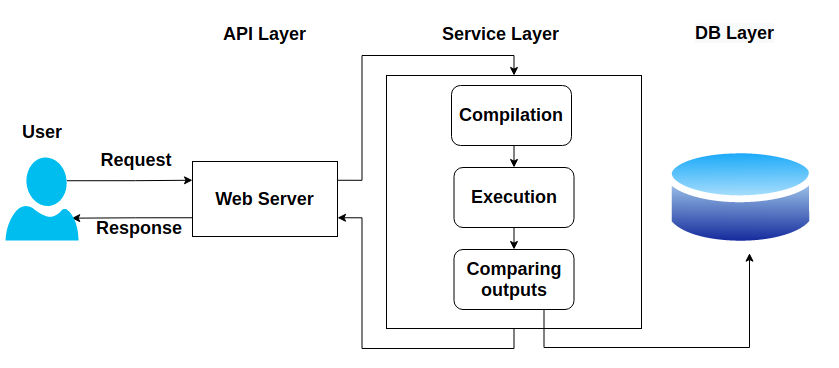
\includegraphics[width=\linewidth]{Images/typical_autograder.png}
  \caption{Typical programming auto-grader architecture}
  \label{typical_auto_grader}
\end{figure}


One major challenge with scalability and performance of the typical programming auto-grader architecture shown in the figure \ref{typical_auto_grader}, is that the processing time of auto-grading session requests depends upon the code the user uploads. Moreover, each user code needs to run against multiple test cases. Let $n$ be the number of test cases on which the code is run and $Test Case Execution Time(i)$ be the execution time required for the $i^{th}$ test case . As shown in the equation \ref{eq:test_case_execution} the total time needed to execute the code is the summation of the time required to execute each test case. Since the resource consumption of different user codes is not the same, the value of $Test Case Execution Time(i)$  will be different among multiple user codes. Therefore the total time required to execute the code will not be the same for different user codes. Hence the processing time of auto-grading session requests is not known and cannot be profiled in any testing setup.

\begin{equation}
  Total Code Execution Time=\sum_{i=1}^{n} Test Case Execution Time(i)
  \label{eq:test_case_execution}
\end{equation}


If the auto-grading session is processed synchronously, the users have to wait till the response for their request is received, which causes a significant number of requests to get a timeout when the request load to the auto-grader is high. Moreover, in general, the users will resend their requests if they don’t get a response within the time they have been patient. Due to which, many users may resend their requests which will further increase the request load to the system and worsen the situation. Hence the auto-grading session requests need to be processed asynchronously. Evalpro is a server-based programming auto-grader, which is a part of Bodhitree. This E-learning application provides extensive features, including in-video quizzes, video quizzes, report grading, discussion forum, and auto-grading of programming assignments \cite{anshul_mtp_thesis}. It has been used extensively in IIT Bombay for the offerings of CS101 computer programming and utilization course for the past few years. In our Evalpro application, the auto-grading session, i.e., compilation, execution, and comparing outputs, is processed asynchronously.


Even though the request processing is asynchronous when the load to the system is very high, the system needs to gracefully handle the high request load, i.e., the system needs to scale its throughput with the request load. But since the system's resources are limited, the system will only support up to a particular request load. After a specific request load, the system's throughput saturates or degrades. Scalability is the ability of the system to scale its performance proportionally by adding resources to the system. If there are any software or hardware bottlenecks, the system won’t scale its performance proportionally by adding resources.

The figure \ref{perf_evalpro_limit} shows Evalpro performance results published in the master’s thesis \cite{anshul_mtp_thesis}, according to which, for 40 CPU cores the throughput of the Evalpro application got flattened at 16 requests per second when the request load is at 1800 users. Also, the CPU utilization didn't exceed 5\%. From these results, it is clear that some application bottlenecks make the Evalpro application’s performance not scale to the high request load. Therefore, identifying the software and hardware bottlenecks limiting the system's performance and increasing the resources corresponding to the identified bottlenecks will make the system gracefully handle the high request load, i.e., The system will scale its performance with the request load.


\begin{figure}[!htb]
            \centering
            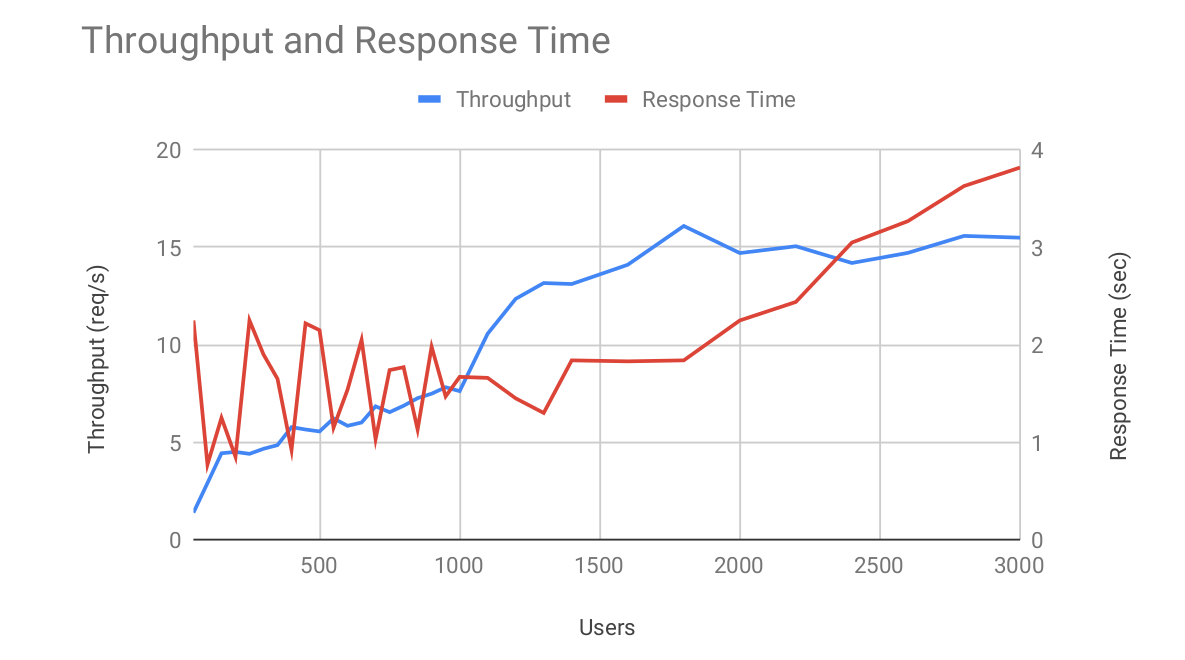
\includegraphics[width=\linewidth]{Images/Performance_limitation.png}
            \caption{Performance limitation of the Evalpro application \cite{anshul_mtp_thesis}}
            \label{perf_evalpro_limit}
\end{figure}

Since the execution of the auto-grading session is non-deterministic, it is impossible to know the resource requirement before handling a certain amount of request load. Hence the scalability of the programming auto-graders is essential to handle the request load gracefully during the peak usage. To achieve the linear scaling of the throughput with CPU cores for our Evalpro application, initially, we performed baseline experiments on our Evalpro application to find the baseline throughput scalability. After that, we performed experiments to identify the software and hardware bottlenecks limiting the application's scalability. We designed solutions to avoid the identified bottlenecks further and make our Evalpro application scale its throughput linearly with the CPU cores.


The rest of the thesis is organized as follows. In Chapter  \ref{motivation_background} we provide background on our Evalpro architecture and baseline experiment setup and further motivate our work using the baseline experiment results. A systematic bottleneck analysis to find the reason for the baseline throughput scalability limitation is briefly described in Chapter \ref{baseline_bottleneck_analysis}. Chapter \ref{horizontal_scalability} describes the Horizontal scalability using Docker swarm and KVM QEMU virtualization technologies and compares the throughput scalability achieved using them with the baseline throughput scalability. Chapter \ref{mongodb_filestorage} describes the usage of MongoDB for storing the files into the database instead of a disk to improve the scalability and compares the throughput scalability achieved using MongoDB with the baseline throughput scalability. In chapter \ref{exp_64}, we perform baseline experiments, the experiments using MongoDB for file storage and the Isolated VM setup experiments on the higher number of CPU cores and compare their throughput scalability. In Chapter \ref{micro_benchmark_exps} we describe two micro benchmarks, i.e., CPU micro benchmark and Evalpro micro-benchmark, which are developed to find the best scalability we can achieve for an Evalpro like application. A low-level bottleneck analysis using the PERF tool to find the reason for throughput scalability limitation in the Evalpro micro benchmark is briefly described in  Chapter \ref{micro_benchmark_bottleneck_analysis}. In chapter \ref{perf_evalpro_application}, we used PERF tool to find the reason for the throughput scalability limitation of the Evalpro application. In chapter \ref{evalpro_recommendation}, we recommend the minimum CPU cache size required for linear scaling of throughput with CPU cores for Evalpro application. Finally, we conclude the thesis in Chapter \ref{conclusion}

\chapter{Background and Motivation}\label{motivation_background}

In the section \ref{tools_technologies}, we provide the overview of  different tools and technologies used in the Evalpro application and the load test experiments to monitor performance of the Evalpro application. In section \ref{evalpro_design}, the current architecture of  the Evalpro application is briefly described. Section \ref{baseline_experiemnt_setup} describes about the experiment setup used for generating the load on the Evalpro application. In the Section \ref{baseline_16}, we describe about the baseline experiment results and further motivates the problem of the throughput scalability with CPU cores for the Evalpro application.


\section{Tools and Technologies}\label{tools_technologies}
This section gives the overview of the following tools and technologies used in the Evalpro application, load test experiments to monitor the performance of it.
\begin{itemize}
    \item Docker
    \item {Docker swarm}
    \item {KVM-QEMU }
    \item {JMeter}
    \item {Linux Utilities}
    \item {MongoDB}
\end{itemize}
\subsection{Docker}
Docker \cite{docker} is a client-server application. As shown in the figure \ref{fig:Docker},  the docker demon is the server that runs natively on the system in Linux. The client part will always be installed natively on the system and sends the commands to the server, i.e., docker daemon, for the execution. Docker Registry stores the docker images. Docker Hub is a public registry in which the docker looks by default for finding the images.
\begin{figure}[!htb]
            \centering
            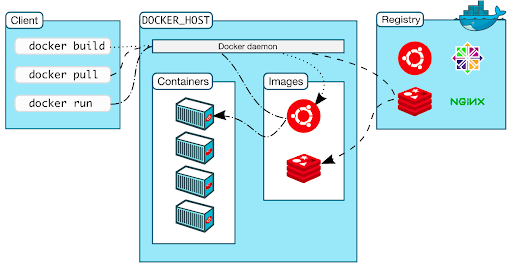
\includegraphics[width=\linewidth]{Images/docker.png}
            \caption{Docker overview \cite{docker_overview}}
            \label{fig:Docker}
\end{figure}
A docker container is a run time construct of a docker image. Docker achieves isolation between the containers using the kernel namespaces feature. The following are some of the kernel namespaces which are used for isolation

\begin{itemize}
    \item {\textbf{PID namespaces}}: The process ID number space is isolated by PID namespaces, which means that processes in different PID namespaces can have the same PID. Thus the containers with different PID namespaces can have their own process ID number space.
    \item {\textbf{Network namespaces}}: The resources related to networking is  isolated by network namespaces, which means that the containers running with different network namespaces can have their own network devices, IP addresses, IP routing tables.
    \item {\textbf{Mount namespaces}}: The file system mount points are  isolated by mount namespaces, which means that the containers running with different mount namespaces can have their own view of the file system hierarchy.
    
\end{itemize}


\subsection{Docker swarm}
Docker swarm \cite{docker_swarm} contains inbuilt cluster management and orchestration features. The cluster management features create a cluster with multiple docker hosts, which act as manager nodes. The multiple docker hosts can be run on a single or multiple physical machines. Docker uses the Raft consensus protocol to maintain the distributed state among multiple docker hosts. As shown in the Figure \ref{fig:docker_swarm}, the Manager node does the cluster management, and the worker nodes execute the container. They won't be involved in cluster management decisions.


Orchestration features in the docker swarm bring automation to container life cycle management, deployment, and scaling. When we specify the desired state, for example, the number of container replicas to be running to the docker swarm, the docker will create the desired state.
\begin{figure}[!htb]
            \centering
            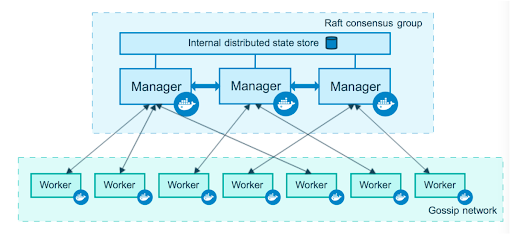
\includegraphics[width=\linewidth]{Images/Docker_swarm.png}
            \caption{Docker swarm  overview \cite{docker_swarm_overview}}
            \label{fig:docker_swarm}
\end{figure}

\subsection{KVM-QEMU}
KVM-QEMU \cite{kvm_qemu} is a hardware-assisted virtualization technique in which the CPU has a special mode of operation called VMX mode to run virtual machines. As shown in the figure \ref{fig:kvm}, QEMU is a Host user-space process that allocates memory for guest VMs. KVM is a kernel driver which switches the CPU to VMX mode to the run guest virtual machine by communicating with QEMU.
\begin{figure}[!htb]
            \centering
            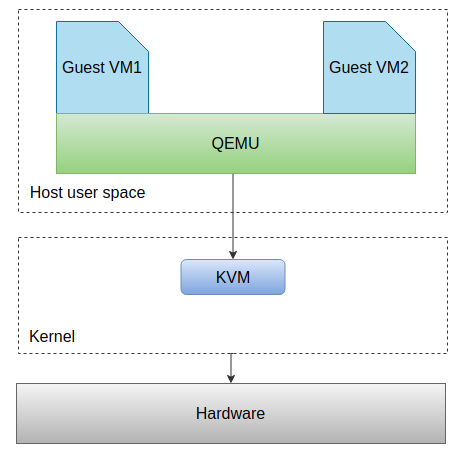
\includegraphics[scale=0.65]{Images/kvm.png}
            \caption{KVM-QEMU overview}
            \label{fig:kvm}
\end{figure}

\subsection{JMeter}
JMeter \cite{jmeter}  is open-source software that is designed to load test applications and measure their performance. JMeter can be used to test the performance of both static and dynamic resources and Web applications. It can be used to simulate a heavy load on a system to measure the maximum load the system can support or measure the overall performance under various load scenarios. It is a multi-threading framework that allows simultaneous sampling of multiple threads, and each thread can run a realistic user session. It also generates the performance metrics in a JSON file and HTML report.

\subsection{Linux Utilities}
During the load test, the server performance metrics are measured using the following  Linux utilities 
\begin{itemize}
    \item iostat \cite{iostat}  for how many bytes are read, and written over an I/O device.
    \item netstat \cite{netstat} for how many bytes are read, and transferred over a network device.
    \item vmstat \cite{vmstat} and mpstat \cite{mpstat} for measuring the CPU utilization.
    \item ps \cite{ps} for finding the  thread-level CPU utilization and CPU time.
    \item iotop \cite{iotop} for finding the thread-level I/O wait percentage.
\end{itemize}

We used PERF\cite{PERF} profiler  tool to measure the occurrence count of various software and hardware events raised during the execution of a workload, such as instructions executed, cache-misses suffered, or branches mispredicted. Per-thread, per-process, per-CPU, and system-wide event counts can be measured using the PERF tool. 

\subsection{MongoDB}
MongoDB \cite{mongo_db} is a NO-SQL database. As shown in the figure \ref{fig:mongodb}, the Database in MongoDB is a set of Collections. A Collection is analogous to a table in SQL databases. It is a set of Documents where each document consists of  data in an unstructured manner, i.e., in the form of key and value pairs. A Document is analogous to a row of a table in SQL databases.
\begin{figure}[!htb]
            \centering
            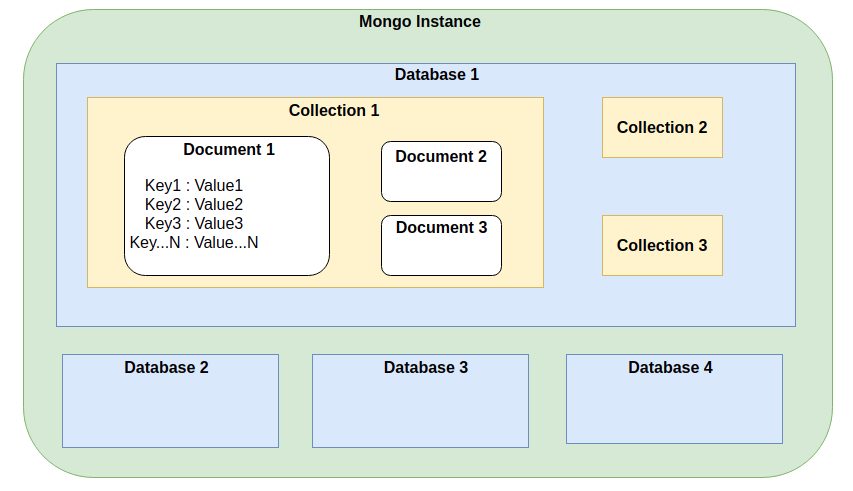
\includegraphics[width=\linewidth]{Images/mongo_db.png}
            \caption{MongoDB overview}
            \label{fig:mongodb}
\end{figure}

\section{Evalpro Design}\label{evalpro_design}
Evalpro is a server-based programming auto-grader application in which auto-grading requests sent by the users are processed at the server. The figure \ref{fig:evalpro_arch} shows the current architecture of the Evalpro application, which runs in the docker  environment. The different components, i.e., Nginx, HAProxy, Postgress, Redis, are isolated by running each component on a separate container. Except for that WSGI, Celery components run on the same container.
\begin{figure}[!htb]
            \centering
            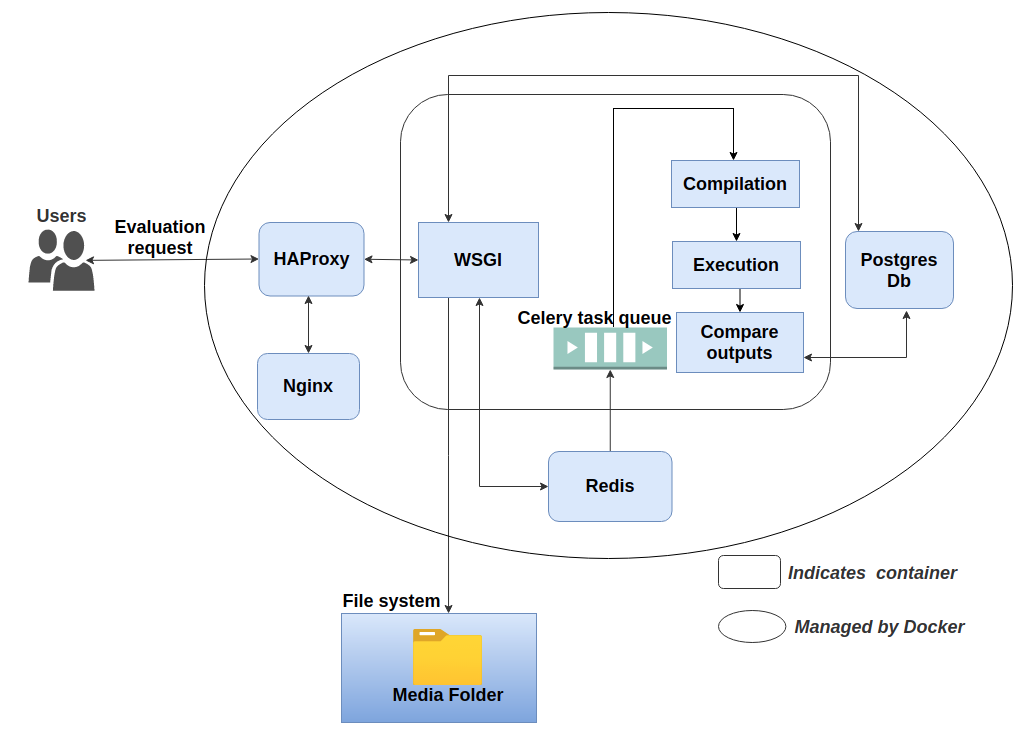
\includegraphics[width=\linewidth]{Images/evalpro_architecture_current.png}
            \caption{Current Evalpro Architecture}
            \label{fig:evalpro_arch}
\end{figure}
\begin{enumerate}
\item {\textbf{WSGI}}: WSGI stands for Web Server Gateway Interface. It behaves as an internal web server, which accepts HTTP requests sent by the load balancer. It contains multiple gunicorn workers, where each worker receives HTTP requests and processes them by sending them into the processing pipeline. After completion of request processing, the response is sent back to the users. Using the File system, it stores the files uploaded by the user in the Media folder .
\item {\textbf{Celery}}:  It executes tasks asynchronously by maintaining a task queue, into which the broker enqueues the messages i.e task-related information. Celery threads will pick the messages from the queue and asynchronously execute the tasks corresponding to the messages. As shown in the figure \ref{fig:evalpro_arch}  celery threads perform the task of auto-grading session i.e compilation, execution, and comparison of outputs asynchronously. After the task is completed, celery informs the message broker about completion.
\item {\textbf{HAProxy}}:  It behaves as a load balancer, which uses the ports exposed by WSGI+Celery replicas to distribute the requests it received among those replicas in a round-robin manner. It also plays the role of an external web server that accepts requests from the external networks and sends the requests for the static content to the static content delivery network(CDN) and the dynamic content to WSGI+Celery replica’s.
\item {\textbf{Redis}}: It acts as a message broker, which enqueues the tasks into the celery task queue. If the task queue is configured to be persistent then while en-queuing a task into the task queue, it also maintains the task information in a file. This will be helpful when some tasks fail to complete due to system crashes, broker will again enqueue the requests related to those tasks to the task queue.
\item {\textbf{Postgres}}:  It is a database server which processes queries related to fetching data from the database and storing data to the database. It maintains application data in a structured manner using tables. The tables are related to each other by foreign keys.
\item {\textbf{Nginx}}: It acts as a static Content Delivery Network (CDN), which process the requests related to the static data, for example fetching HTML, and JavaScript files.

\end{enumerate}

Using this architecture we have performed baseline experiments to find the current scalability of our Evalpro application.  Section \ref{baseline_experiemnt_setup} i.e the next section discuss about our experiment setup to perform baseline experiments. Section \ref{baseline_16} further motivates our work by discussing the baseline experiment results.

\section{Experiment setup}\label{baseline_experiemnt_setup}
We have designed a realistic user session using JMeter to perform experiments on our Evalpro application.
\begin{figure}[!htb]
  \centering
  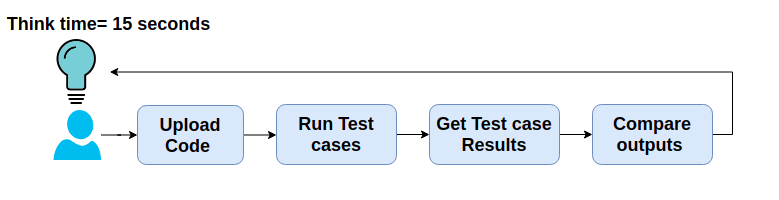
\includegraphics[width=\linewidth]{Images/user_session.png}
  \caption{JMeter user session}
  \label{user_session}
  
\end{figure}
As shown in the figure \ref{user_session}, the user session is simulated with JMeter consists of following steps
\begin{itemize}
\item {\texttt{Upload Code}}: Upload the code in a file by clicking the upload button from the User Interface.
 \item {\texttt{Run Test cases}}: Compiles the user code uploaded in the above step and runs the executable file on the available test cases.
\item {\texttt{Get Test case Results}}: After the test cases, execution gets completed in the above step. A page will be displayed to the user which shows the results of the test cases execution.
\item {\texttt{Compare outputs}}: Using the page displayed in the above step, for each test case the output of the uploaded code is compared with the actual output.
\item {\texttt{Think time}}: It is the time for which the user waits before starting the user session for the next time. We have configured the think time to be 15 seconds for our experiments.
\end{itemize}
\begin{figure}[!htb]
  \centering
  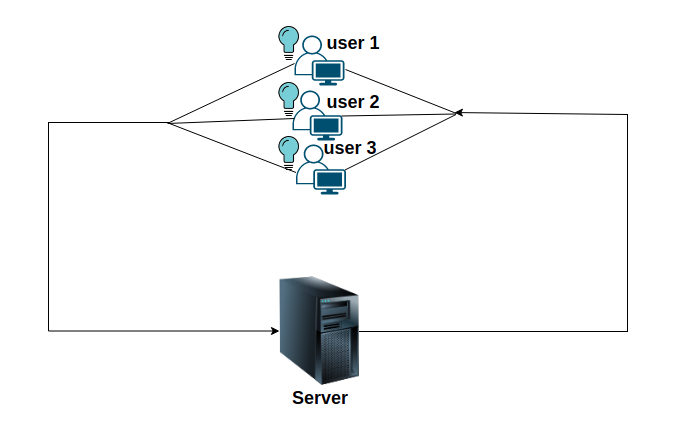
\includegraphics[width=\linewidth]{Images/closed_loop.png}
  \caption{Closed load system}
  \label{closed_system}
\end{figure}

\begin{table}
  \begin{tabular}{|c|p{9em}|c|c|c|c|c|}
    \hline
    Type&CPU&Cores&Memory&L3 cache&L2 cache&L1 cache\\
    \hline
    Server & Intel\textsuperscript{R} Xeon\textsuperscript{R} CPU E5-2650 v2 @ 2.60GHz& 16&16GB&20MB&256KB&32KB\\
    \hline
    Client & AMD Opteron\textsuperscript{TM} Processor 6212 & 16&16GB&6MB&2MB&64KB\\
  \hline
\end{tabular}
\caption{Hardware specifications for Baseline-16 Experiments}
  \label{tab:hardware}
\end{table}

As shown in the figure  \ref{closed_system}, a closed load system is created in which  the above described user session is run simultaneously by creating multiple users using JMeter  on the client machine and the Evalpro application is run on the sever machine which accepts requests sent by multiple users from the client machine. The generation of the load from the client is configured to run for 5 minutes using JMeter. During the load test, server performance metrics are collected using the various Linux utilities i.e vmstat, mpstat, iostat, iotop, netstat and ps.

The figure \ref{loag_gen_measure} shows the Load generation and performance measurement infrastructure, in which the load generation script , i.e.,  loadtest.sh, runs in the client machine, which uses JMeter to generate  load on the Evalpro application running in the server machine. It also triggers the background execution of Linux utilities in the server machine. The Linux utilities collect server performance metrics , i.e., CPU utilization, disk utilization, and network bandwidth of the Evalpro application. After the load test is completed, files logged in the server by Linux utilities have been automatically transferred to the client machine using the experiment timestamp. JMeter collects the request throughput and latency. At the end, all the required files for the performance measurement will be stored in a folder on the disk in the client machine.

\begin{figure}[!htb]
  \centering
  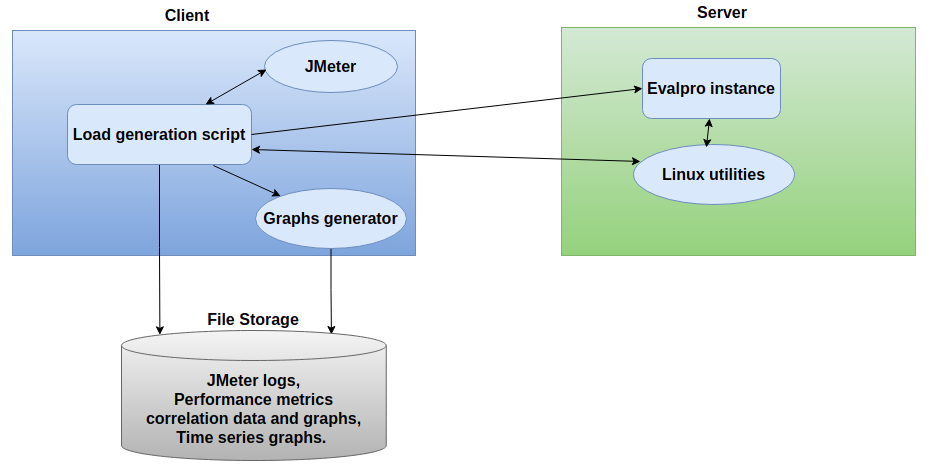
\includegraphics[width=\linewidth]{Images/Measurement_infrastructure.png}
  \caption{Load generation and Performance measurement infrastructure}
  \label{loag_gen_measure}
\end{figure}




The table \ref{tab:hardware} shows various hardware specifications of the client and the server machines. Using this experiment setup, we have performed the baseline experiments to find the current scalability of the Evalpro application. The next section briefly describes the baseline experiments and further motivates our work using the results.

\section{Baseline - 16}\label{baseline_16}

As shown in the figure \ref{baseline_16_setup}, in our baseline experiments for an Evalpro instance we used 16 CPU core sever, shown in the table \ref{tab:hardware} and used single a WSGI+Celery replica. To avoid the obvious bottlenecks, we have configured the number of celery threads equal to the number of CPU cores, the number of Postgres connections to 10000, a relatively higher number compared to the default value of 100. We have performed experiments by altering the number of CPU cores available.
\begin{figure}[!htb]
  \centering
  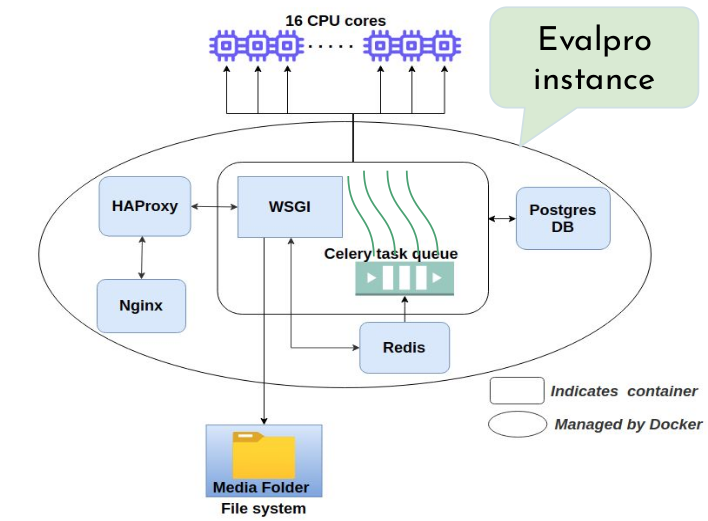
\includegraphics[width=\linewidth]{Images/Baseline-16.png}
  \caption{Baseline-16 experiment setup}
  \label{baseline_16_setup}
\end{figure}

The observed throughput is the throughput we observed from our experiments, we define the maximum throughput observed with $N$ CPU cores as $Throughput_{max}(N)$. The ideal throughput with $N$ CPU cores is the desired throughput, which is equal to $N*Throughput_{max}(1)$. The observed value of $Throughput_{max}(1)$ is 0.3 requests per second. As shown in the figure \ref{baseline_throughput_plot}, when the number of CPU cores $N$ increases, the maximum throughput observed with $N$ CPU cores, $Throughput_{max}(N)$ increases linearly up to $N=8$ CPU cores. When the number of CPU cores $N>8$, then the difference between the values of the observed  $Throughput_{max}(N)$  and the ideal throughput with $N$ CPU cores is significantly high i.e the throughput is not scaling linearly.


\begin{figure}[!htb]
  \centering
  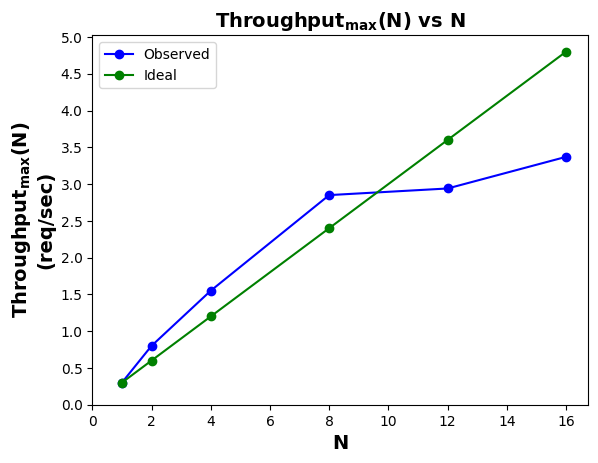
\includegraphics[width=\linewidth]{Images/Baseline-16_throughput.png}
  \caption{Baseline-16 Throughput plot}
  \label{baseline_throughput_plot}
\end{figure}


\begin{figure}[!htb]
  \centering
  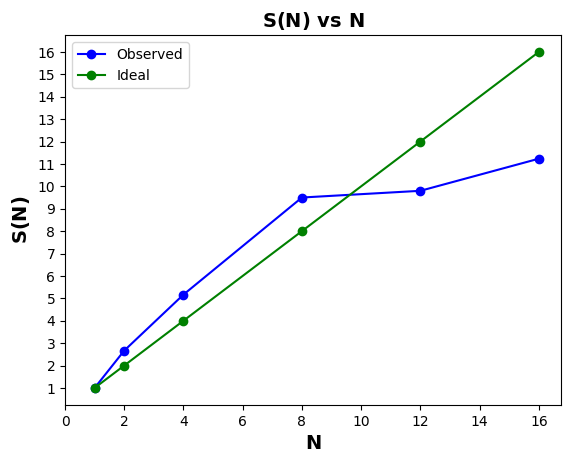
\includegraphics[width=\linewidth]{Images/Baseline-16_scalability.png}
  \caption{Baseline-16 Throughput Scalability plot}
  \label{baseline_scalability_plot}
\end{figure}

To measure how well the scaling of the throughput is happening we define scalability factor. As shown in the equation \ref{eq:1}, the scalability factor for $N$ CPU cores is  $S(N)$, which is equal to the ratio of the maximum throughput observed with $N$ CPU cores,  $Throughput_{max}(N)$ and the maximum throughput observed with a single CPU core $Throughput_{max}(1)$.
\begin{equation}
  S(N)=\frac{Throughput_{max}(N)}{Throughput_{max}(1)}
  \label{eq:1}
\end{equation}

For our baseline experiments we have calculated $S(N)$ value for different values of $N$, the number of CPU cores. Using the figure \ref{baseline_scalability_plot}, we have compared the observed scalability factor with the ideal scalability factor. The observed scalability factor for 16 CPU cores is 11.23, but the ideal value of S(16) is 16, which is shown in the table \ref{tab:baseline_16_results}. By these results, it is clear that the throughput scalability of the Evalpro application is not scaling proportionally with increase in the number of CPU cores. To get the linear scaling of the throughput  $S(N)$ should be as close as $N$.

\begin{table}[!htb]
    \centering
  \begin{tabularx}{\textwidth}{|X|X|}
    \hline
    \makecell{$Throughput_{max}(1)$ \\ (req/sec)} & \makecell{0.3}\\
    \hline
    \makecell{$Throughput_{max}(8)$ \\ (req/sec)} & \makecell{2.85}\\
    \hline
    \makecell{$Throughput_{max}(16)$ \\ (req/sec)} & \makecell{3.44}\\
    \hline
    \makecell{Ideal $Throughput_{max}(16)$ \\ (req/sec)} & \makecell{4.8}\\
    \hline
    \makecell{$S(16)$} & \makecell{11.23}\\
    \hline
\end{tabularx}
\caption{Baseline - 16 Experiments results}
  \label{tab:baseline_16_results}
\end{table}

In general, the scalability limitation of an application is due to some underlying bottlenecks in the closed load system which make the application's performance not to  scale proportionally with increase in the hardware resources. Therefore we hypothesize that there are some bottlenecks that are limiting the scalability of the Evalpro application. Some examples of bottlenecks include insufficient threads for processing, lock contention of software, and hardware resources. To find the bottlenecks and improve the current baseline scalability, we have done bottleneck analysis on the baseline experiment setup by tuning different software components of the Evalpro application. The next chapter briefly describes the baseline bottleneck analysis on the Evalpro application.


\chapter{Baseline Bottleneck Analysis}\label{baseline_bottleneck_analysis}

As shown in the previous chapter, the throughput of the Evalpro application didn't scale proportionally with the increase in the number of CPU cores. Based on our hypothesis at the end of the previous section that some bottlenecks are limiting the scalability of the Evalpro application, in this section, we have done bottleneck analysis on the Evalpro application to find the reason for the limitation in the current scalability and improve it. To find the bottlenecks and improve the current baseline scalability, we have performed the following experiments by tuning the performance parameters of different software components.
\begin{itemize}
    \item
    Increasing gunicorn workers
    \item
    Modifying celery threads
    \item
    Setting CPU affinities to celery threads
    \item
    Disabling writing to log files
    \item
    Modifying Celery Prefetch multiplier
    \item
    Increasing celery broker pool limit
    \item
    Using transient celery queue
\end{itemize}


\section{Increasing gunicorn workers:}
Gunicorn workers are part of WSGI, which accepts HTTP requests sent by the users and send them into the execution pipeline. The number of gunicorn workers for the baseline experiments is 10. We tried to modify the number of gunicorn workers to see improvement in $S(N)$ for $N>8$. When the number of CPU cores $N$ is equal to 16 we have modified the number gunicorn workers configuration. As shown in the figure \ref{gunicorn_plot} when the number of gunicorn workers increased the value of $S(16)$, almost remains constant. By this we can say that tuning the number of gunicorn workers doesn't improve  $S(N)$ for $N>8$.
\begin{figure}[!htb]
  \centering
  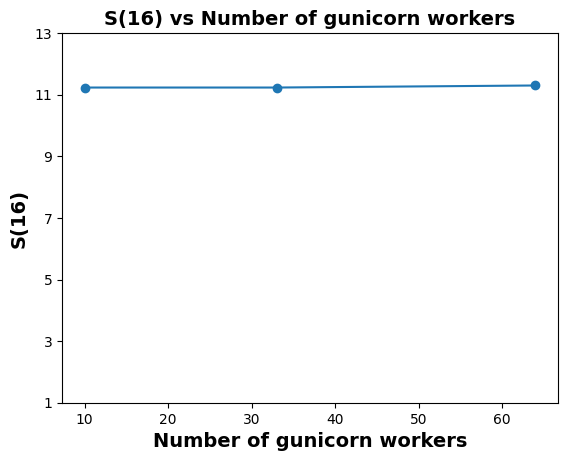
\includegraphics[width=\linewidth]{Images/gunicorn_workers.png}
  \caption{Tuning Gunicorn workers}
  \label{gunicorn_plot}
\end{figure}

\section{Modifying celery threads:}
Celery threads pick the tasks en-queued into the celery queue by the message broker, Redis, and execute those tasks asynchronously. In our Evalpro application, the task of the auto-grading session is performed asynchronously by the celery threads. The number of celery threads for the baseline experiments equals $N$, the number of CPU cores. We tried to modify the number of celery threads to see improvement in $S(N)$ for $N>8$. When the number of CPU cores N equals 16, we have modified the number of celery threads. 

As shown in the figure \ref{celery_plot}, when the number of celery threads are less than 16, S(16) value is less than the baseline value of 11.2. Moreover, from the CPU utilization plot in the figure \ref{celery_cpuutil} it is clear that  when the number of celery threads is less than $N$, they are becoming the bottleneck  making the CPU not utilized completely. When the celery threads count is greater than 16, S(16) value almost remained constant. By this we can say that increasing the celery threads count beyond $N$ doesn't improve $S(N)$.
\begin{figure}[!htb]
  \centering
  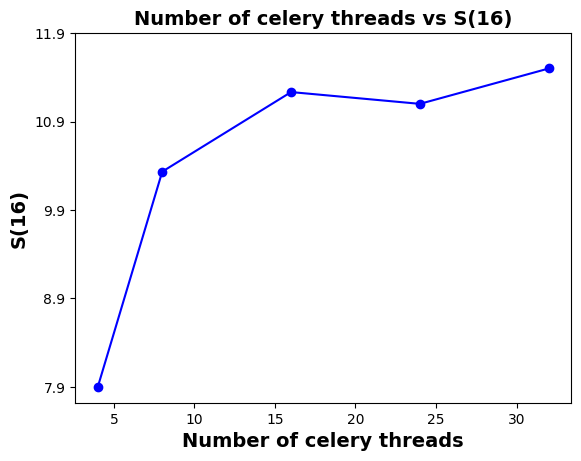
\includegraphics[width=\linewidth]{Images/celery_threads_scalability.png}
  \caption{Number of Celery threads vs Scalability factor for 16 CPU cores}
  \label{celery_plot}
\end{figure}

\begin{figure}[!htb]
  \centering
  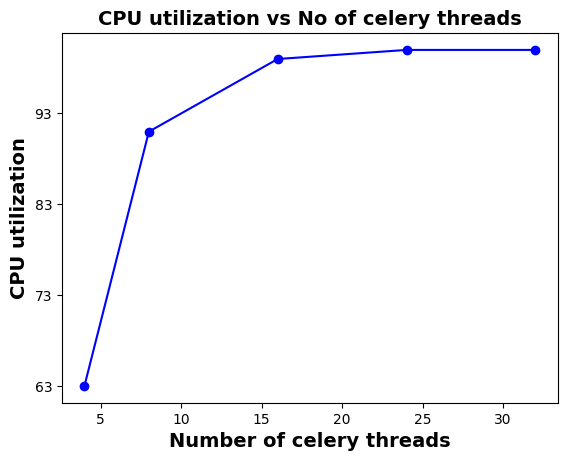
\includegraphics[width=\linewidth]{Images/celery_threads_utilization.png}
  \caption{Number of Celery threads vs CPU Utilization}
  \label{celery_cpuutil}
\end{figure}

\section{Setting CPU affinities to celery threads:}
When each thread is run on a different CPU core, there will be less inter-core contention. Due to this, we hypothesized that setting CPU affinities to celery threads will improve  $S(N)$ for $N>8$. When the number of CPU cores $N$ is equal to 16, using the Linux taskset command we have pinned each celery thread to a CPU core but observed no improvement in $S(16)$.
\section{Disabling writing to log files:}
During the processing of requests by the Evalpro application, useful metadata regarding request processing is logged into files by the application at different stages of processing. We hypothesized that due to logging CPU is doing work that is not useful. so, to see improvement in $S(N)$ for $N>8$, we disabled writing to gunicorn access log and celery log files. After disabling logging, we performed experiment when the number of CPU cores $N$ is equal to 16 and measured $S(16)$ value, which came out to be 11, very close to the baseline value of 11.2. By this, we can say that disabling writing to log files doesn’t improve $S(N)$ for $N>8$.
\section{Modifying celery prefetch multiplier:}
Prefetch multiplier is the number of tasks each celery thread fetches at a time from the queue and keeps in the memory instead of going to queue and fetching the task every time. For our baseline experiments, the prefetch multiplier value is 4. We have modified the value of the prefetch multiplier to see improvement in $S(N)$ for $N>8$. When the number of CPU cores $N$  equals 16, we have modified the value of the prefetch multiplier. 

As shown in the figure \ref{prefetch_multiplier_plot} when the value of the prefetch multiplier changed, the value of $S(16)$,  almost remains constant. By this, we can say that tuning the value of the prefetch multiplier doesn’t improve   $S(N)$ for $N>8$.
\begin{figure}[!htb]
  \centering
  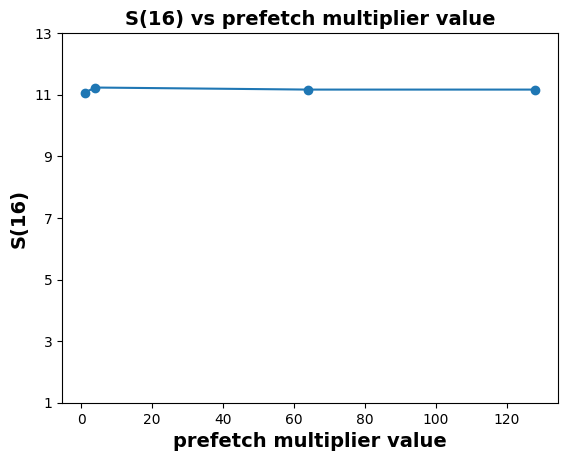
\includegraphics[width=\linewidth]{Images/prefetch_multiplier.png}
  \caption{Tuning Celery Prefetch multiplier}
  \label{prefetch_multiplier_plot}
\end{figure}
\section{Increasing celery broker pool limit}
Broker pool limit is the number of connections celery keeps open instead of creating a new connection for every task en-queued into the celery task queue by the message broker, Redis. The celery broker pool limit for the baseline experiments is 10. We tried to modify this value to see improvement in $S(N)$ for $N>8$. When the number of CPU cores $N$ is equal to 16 we have modified the broker pool limit configuration. 

As shown in the figure \ref{broker_pool_limit} when the broker pool limit has increased the value of $S(16)$, almost remains same as baseline $S(16)$ value. By this, we can say that tuning the broker pool limit doesn't improve $S(N)$ for $N>8$.
\begin{figure}[!htb]
  \centering
  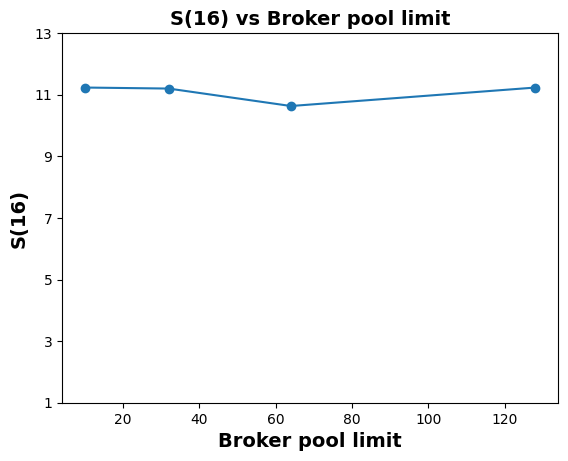
\includegraphics[width=\linewidth]{Images/broker_limit.png}
  \caption{Tuning Broker pool limit}
  \label{broker_pool_limit}
\end{figure}
\section{Using transient celery queue}
By default celery queue is persistent, the task information is logged
into a file by the message broker,Redis when the task is en-queued into the celery task queue. Persistent queues are useful when the system crashes occur, the broker will  use the file to en-queue the failed tasks into the celery 
task queue. To see the improvement in $S(N)$ for $N>8$, we have made the celery task queue transient when the number of CPU cores $N$ is equal to 16 but observed no improvement in $S(16)$. By this we can say that using transient celery queue doesn't improve  $S(N)$ for $N>8$.


From the results of the above experiments, it is clear that tuning the performance parameters of different software components didn't improve the current baseline scalability. We also have observed that when the throughput achieved is maximum, the CPU utilization of the server is around 90-100\% . Therefore we came to the conclusion that there is no  are no application bottlenecks, from which we came to the hypothesis that, the isolation between the software, and hardware resources improves scalability. So, we have  horizontally scaled the Evalpro application to achieve a better scalability factor, $S(N)$ for $N>8$.  The next chapter briefly describes the usage of horizontal scalability for our Evalpro application.



\chapter{Horizontal Scalability} \label{horizontal_scalability}
Horizontal scalability is the ability of the system to scale its performance when a new application replica is added which consists of a new set of hardware resources i.e CPU, memory, or disk. The load balancer will distribute the load across multiple replicas. We have used two different virtualization techniques, Containers and Virtual machines for Horizontal scalability.
\section{Horizontal scaling with Containers}
Docker has inbuilt cluster management and orchestration framework, docker swarm. As shown in the figure \ref{docker_swarm}, using docker swarm multiple replicas of WSGI+Celery container replicas are created with each replica assigned with different CPU cores. The HAProxy will balance the request load from the users in a round-robin manner across different WSGI+Celery replicas. Moreover, each container replica will have a different PID namespace. Thus the isolation with containers is more compared to the baseline experiments. 

As shown in the figure \ref{docker_swarm}, when the number of CPU cores $N$ is equal to 16, 4 WSGI+Celery replicas are created with each replica assigned with 4  different CPU cores. Using this experiment setup, we performed experiments and found that the maximum throughput observed with 16 CPU cores, $Throughput_{max}(16)$ is 3.4 requests per second and the  scalability factor with 16 CPU cores, $S(16)$ value is 11.33. We have compared these results with the Baseline results. As shown in the table \ref{tab:baseline_container}, values of $Throughput_{max}(16)$ and $S(16)$ observed by scaling horizontally with 4 WSGI+Celery container replicas is almost same the baseline values of 3.37 requests per second and 11.2, respectively. By this, we can say that scaling the Evalpro application horizontally using containers doesn't improve  $S(N)$ and $Throughput_{max}(N)$ for $N>8$.
\begin{figure}[!htb]
  \centering
  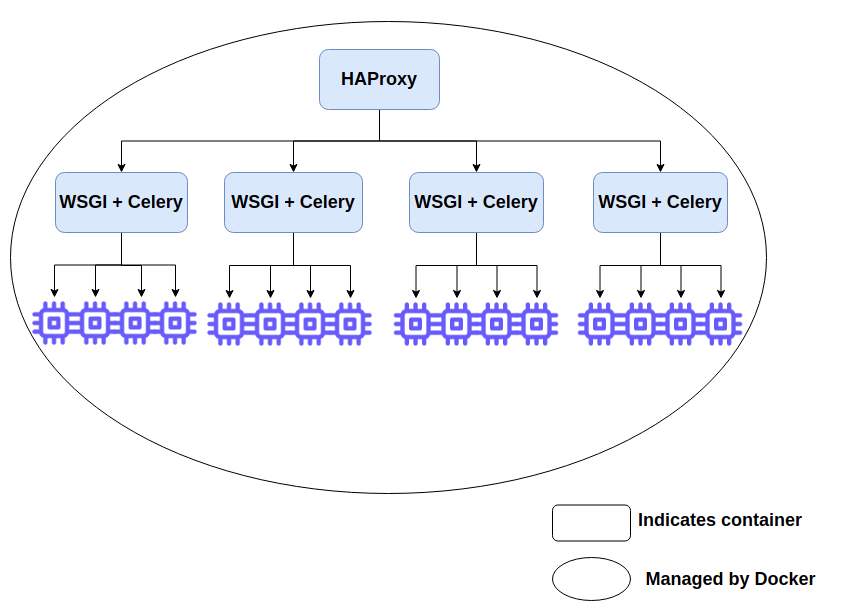
\includegraphics[width=\linewidth]{Images/docker-swarm_scaling.png}
  \caption{Horizontal scaling with docker}
  \label{docker_swarm}
\end{figure}


    \begin{table}[!htb]
    \centering
  \begin{tabularx}{\textwidth}{|X|X|X|}
    \hline
    &\makecell{Baseline}&\makecell{Docker swarm}\\
    \hline
    \makecell{$Throughput_{max}(1)$\\(req/sec)} & \makecell{0.3} & \makecell{0.3}\\
    \hline
    \makecell{$Throughput_{max}(16)$\\(req/sec)} & \makecell{3.37} & \makecell{3.4}\\
    \hline
    \makecell{Ideal $Throughput_{max}(1)$\\(req/sec)} & \makecell{4.8} & \makecell{4.8}\\
    \hline
    \makecell{$S(16)$} & \makecell{11.23} & \makecell{11.3}\\
  \hline
\end{tabularx}
\caption{Baseline vs Container based Scaling}
  \label{tab:baseline_container}
\end{table}




\section{Horizontal scaling with Virtual Machines}
We have used KVM-QEMU, which is a hardware assisted virtualization technique for scaling horizontally using Virtual machines. Using KVM-QEMU hypervisor multiple VMs can be created with each VM assigned with a different set of CPU cores. Moreover, each VM can get its own share of the RAM and the Disk. Thus the isolation with VMs is more than with containers and the baseline experiments. The isolation of the hardware resources between VMs is managed by the KVM-QEMU hypervisor.
\subsection{Completely Isolated setup}\label{isolated_setup_16}
As shown in the figure \ref{isolated_vm}, when the number of CPU cores $N$ is equal to 16, 2 VMs are created with each replica assigned with 8 different CPU cores, 8GB RAM, and 30GB hard disk. Evalpro instance is run on each VM in a completely isolated manner. Using this experiment setup, we have performed experiments and found that the maximum throughput observed with 16 CPU cores, $Throughput_{max}(16)$ is 4.45 requests per second and the  scalability factor with 16 CPU cores, $S(16)$ value is 14.8. All the CPU cores in both VMs have been completely utilized. We have compared these results with the baseline results. As shown in the table \ref{tab:baeline_isolated_vm}, values of $Throughput_{max}(16)$ and $S(16)$ is significantly more than the baseline values of 3.37 requests per second and 11.2, respectively. But in this setup, each Evalpro instance has a separate Postgres database which constitutes the following limitations 
\begin{figure}[!htb]
  \centering
  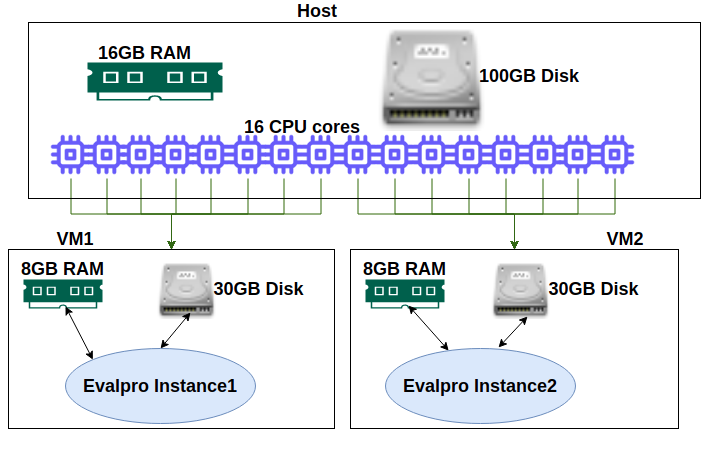
\includegraphics[width=\linewidth]{Images/isolated_vm.png}
  \caption{Completely Isolated VM setup}
  \label{isolated_vm}
\end{figure}


 \begin{table}[!htb]
    \centering
  \begin{tabularx}{\textwidth}{|X|X|X|}
    \hline
    &\makecell{Baseline}&\makecell{Isolated VM setup}\\
    \hline
    \makecell{$Throughput_{max}(1)$\\(req/sec)} & \makecell{0.3} & \makecell{0.3}\\
    \hline
    \makecell{$Throughput_{max}(16)$\\(req/sec)} & \makecell{3.37} & \makecell{4.45}\\
    \hline
    \makecell{Ideal $Throughput_{max}(1)$\\(req/sec)} & \makecell{4.8} & \makecell{4.8}\\
    \hline
    \makecell{$S(16)$} & \makecell{11.23} & \makecell{14.5}\\
  \hline
\end{tabularx}
\caption{Baseline vs Completely Isolated VM setup}
  \label{tab:baeline_isolated_vm}
\end{table}


\begin{itemize}
    \item 
    Separate user-related data should be maintained for each Evalpro instance and the load balancer needs to maintain information about to which instance it has to forward the request so that the user gets the correct response.
    \item
    Moreover when the request load is high i.e the VMs are completely utilized, adding a new VM to scale the performance of the system, requires migration of the part of user data to the new VM from the old VMs, which is a very complex as the tables in Postgres database are related to each other by the foreign keys.
\end{itemize}

Due to the above limitations, it is very complex and infeasible to use an Isolated VM setup. So, we have shared the user-related data, and files among multiple VMs so that the load balancer need not maintain request to instance mapping, it can distribute the user requests to multiple VMs in a round-robin manner and new VMs can be added to scale the performance of the system without any requirement of the migration of the user data. The next section briefly describes this experimental setup.
\subsection{User Data and Files sharing setup}
As shown in the figure \ref{shared_vm}, the Postgres Database and the Media folder which consists of the files uploaded by the user for running code is shared among the two VMs. The media folder is placed in the Host machine and mounted on both the VMs so that both the VMs can share the Media folder to store user uploaded files. Using this experiment setup, we have performed experiments and found that the maximum throughput observed with 16 CPU cores, $Throughput_{max}(16)$ is 2.78 requests per second and the  scalability factor with 16 CPU cores, $S(16)$ value is 9.26. Moreover all the CPU cores in both VMs have not been completely utilized i.e 80\% utilized.  We have compared these results with the baseline results. As shown in the table \ref{tab:baseline_shared_vm}, values of $Throughput_{max}(16)$ and $S(16)$ is less than the the baseline values of 3.37 requests per second and 11.2, respectively.
\begin{figure}[!htb]
  \centering
  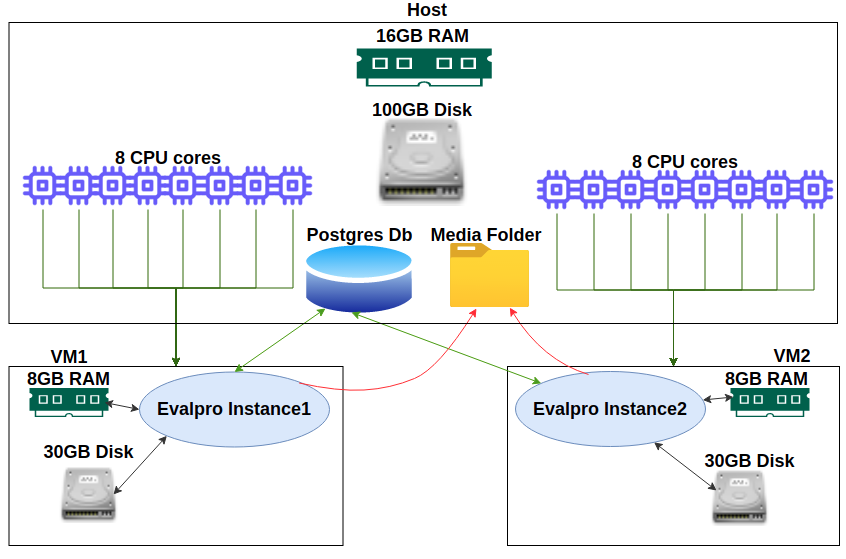
\includegraphics[width=\linewidth]{Images/shared_vm.png}
  \caption{User data and Files sharing VM setup}
  \label{shared_vm}
\end{figure}


\begin{table}[!htb]
    \centering
  \begin{tabularx}{\textwidth}{|X|X|X|}
    \hline
    &\makecell{Baseline}&\makecell{Data and Files sharing \\VM setup}\\
    \hline
    \makecell{$Throughput_{max}(1)$\\(req/sec)} & \makecell{0.3} &\makecell{ 0.3}\\
    \hline
    \makecell{$Throughput_{max}(16)$\\(req/sec)} & \makecell{3.37} & \makecell{2.78}\\
    \hline
    \makecell{Ideal $Throughput_{max}(1)$\\(req/sec)} &\makecell{4.8} & \makecell{4.8}\\
    \hline
    \makecell{$S(16)$} & \makecell{11.23} & \makecell{9.6}\\
  \hline
\end{tabularx}
\caption{Baseline vs User data and Files sharing VM setup}
  \label{tab:baseline_shared_vm}
\end{table}





Thus with the above experiment results, we came to the conclusion that with the User data and Files sharing VM setup there are some bottlenecks that are making the Evalpro application not to scale. The next section briefly describes about empirically finding  the reason for scalability limitation  with this experimental setup.

\section{Bottleneck analysis of Data, Files sharing VM setup }
To find the  the reason for scalability limitation  of the Evalpro application with the Data, Files sharing VM setup setup  described in the above section, in this section we empirically performed bottleneck analysis. We have divided the current user session shown in the figure \ref{user_session}, into the following parts.
\begin{enumerate}
    \item {\texttt{Without Upload:}} As shown in the figure \ref{without_upload_session}, this user session consists of all the steps in the current user session shown in the figure  \ref{user_session}, except the step in which the user uploads the code. Since there is no file upload,  we have reduced the think time of the user to 8 seconds from 15 seconds.
    \begin{figure}[!htb]
  \centering
  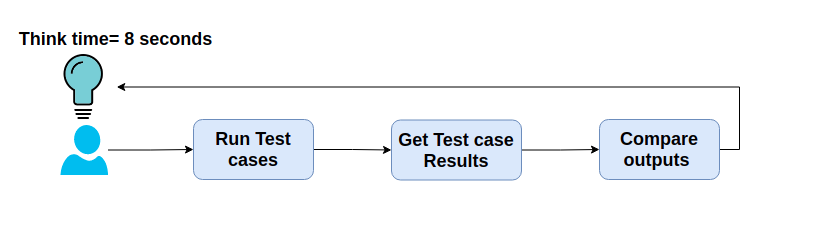
\includegraphics[width=\linewidth]{Images/with_out_upload_session.png}
  \caption{User session without upload}
  \label{without_upload_session}
\end{figure}
    \item {\texttt{Only Upload:}} As shown in the figure \ref{upload_session}, this user session only consists of the step where the user uploads the code. We have configured the user think time to be the same as the  current user session, shown in the figure \ref{user_session} i.e 15 seconds.
    \begin{figure}[!htb]
  \centering
  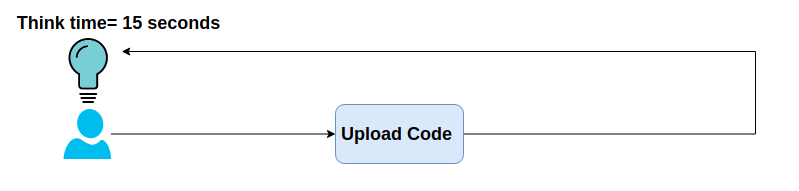
\includegraphics[width=\linewidth]{Images/only_upload_session.png}
  \caption{User session with only upload}
  \label{upload_session}
\end{figure}
\end{enumerate}




Using the \texttt{Without Upload}  user session shown in the figure \ref{without_upload_session}, we have performed experiments on a single CPU core. The maximum throughput achieved on a single CPU core, $Throughput_{max}(1)$ was observed to be 1.35 requests per second. With the Data, Files sharing  VM  setup shown in the figure \ref{shared_vm}, we performed experiments and found that the maximum throughput achieved on the 16 CPU cores, $Throughput_{max}(16)$ to be 17.31 requests per second. We calculated $S(16)$, the scalability factor with 16 CPU cores using the equation \ref{eq:1}, by which  the $S(16)$ value is 13, which is close to the ideal $S(16)$ value of 16.

Same experiments described above are performed using \texttt{Only Upload} user session shown in the figure \ref{upload_session}, in which the single CPU core maximum throughput,  $Throughput_{max}(1)$ was observed to be 1.26 requests per second.  With the Data, Files sharing  VM  setup shown in the figure  \ref{shared_vm}, the  maximum throughput with 16 CPU cores, $Throughput_{max}(16)$  was observed to be 5.91 requests per second. Therefore by using the equation \ref{eq:1}, the Scalability factor with 16 CPU cores, $S(16)$ value is 4.71.


\begin{figure}[!htb]
  \centering
  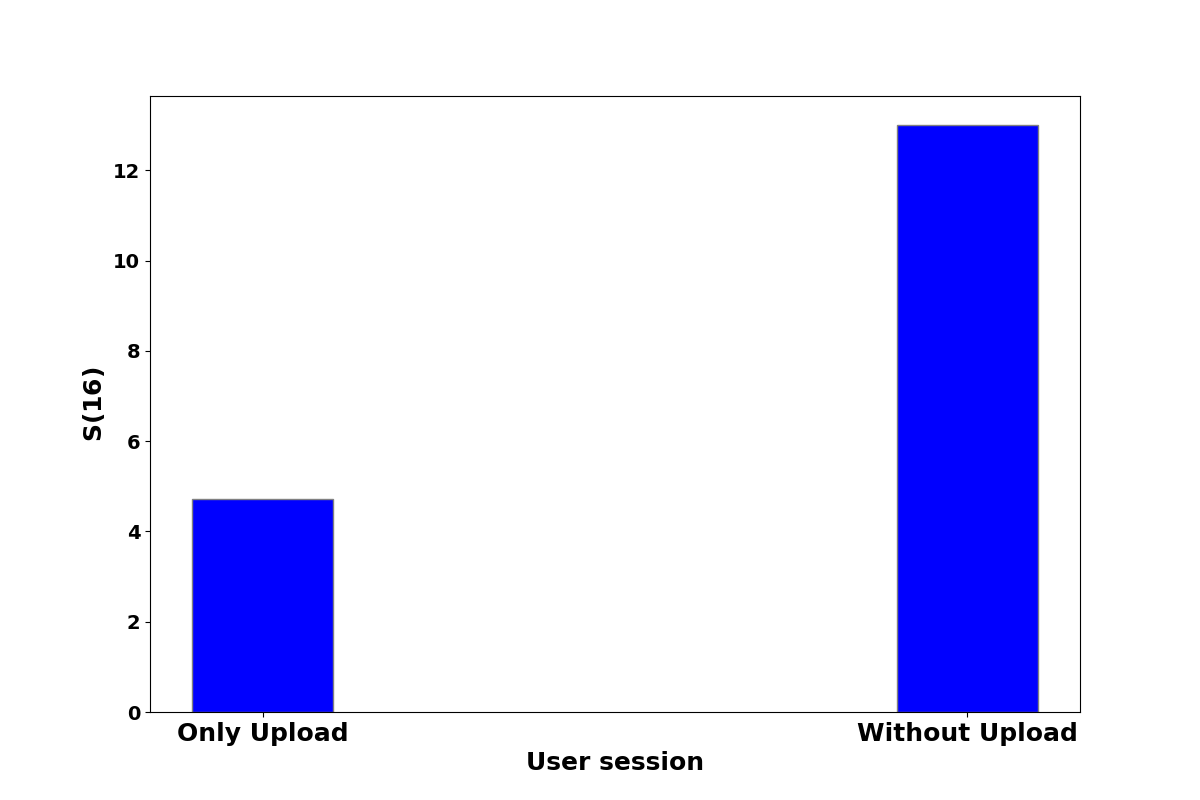
\includegraphics[width=\linewidth]{Images/upload_vs_without_upload.png}
  \caption{Scalability for different user sessions}
  \label{compare_user_sessions}
\end{figure}

By comparing the $S(16)$  value calculated above for \texttt{Without Upload} and  \texttt{Only Upload} user sessions shown in the figure  \ref{compare_user_sessions}, we observed that for \texttt{Only Upload} user session the scalability  of the Evalpro application is very less compared to \texttt{Without Upload}. Moreover the CPU utilization of the server for  \texttt{Only Upload} user session  didn't exceed  35\%, which also confirms that uploading file is the bottleneck. From these results we came to the conclusion that for the combined user session shown in the figure \ref{user_session}, using the shared VM setup shown in the figure \ref{shared_vm}, file upload is becoming the bottleneck because uploading a file in the Media folder which is in the host requires each VM to make a context switch to the Host and upload file in the Media folder, which is a significant overhead

Therefore we hypothesize that with the shared VM setup shown in the figure \ref{shared_vm},  using the database to store the uploaded files instead of the disk will improve the scalability factor $S(N)$ for $N>8$. There is no need for VMs to make a context switch to the host to upload a file when the files are stored in the database and shared between VMs. So, we used the MongoDB database to store the uploaded files. The following section briefly describes the experiments performed on the Evalpro application using MongoDB to store the files uploaded by the user.


\chapter{MongoDB for File Storage}\label{mongodb_filestorage}
MongoDB is a NO-SQL database. It stores data in an unstructured manner using key and value pairs. Based on our hypothesis from the above experiments, we used MongoDB to store the user uploaded files. As shown in the figure \ref{architecture_mongo}, we have modified the current Evalpro architecture shown in the figure \ref{fig:evalpro_arch} by replacing the file system with MongoDB to store the files uploaded by the user. We have performed experiments on this new Evalpro architecture to see the improvement in in $S(N)$ for $N>8$. We  have changed the User Data and Files sharing setup shown in the figure \ref{shared_vm} by replacing the Media folder with MongoDB. The User Data and Files sharing setup with MongoDB  is shown in the figure \ref{shared_vm_mongo}.

\begin{figure}[!htb]
  \centering
  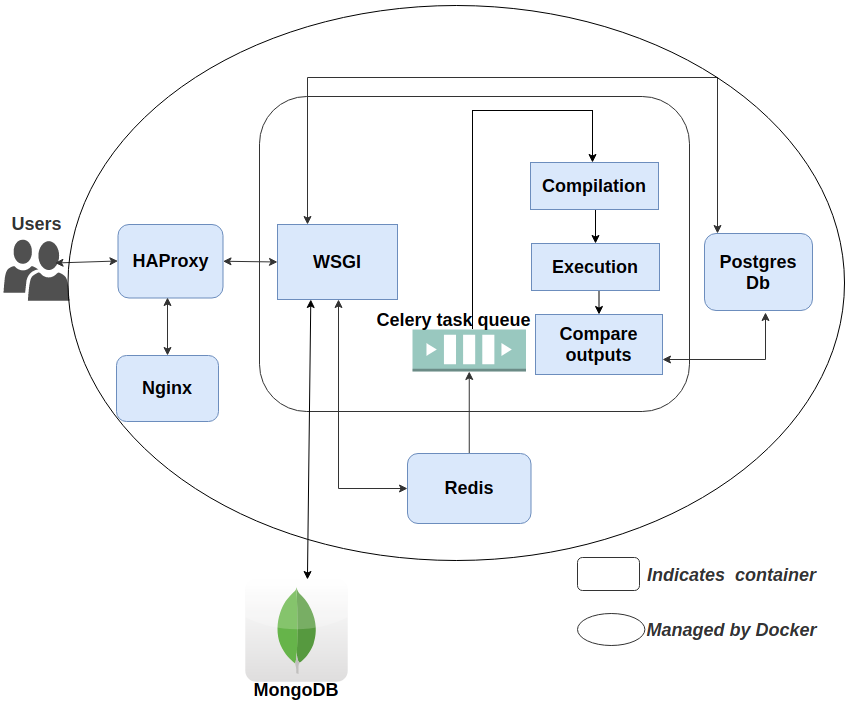
\includegraphics[scale=0.45]{Images/evalpro-architecture_mongo.png}
  \caption{Evalpro new architecture}
  \label{architecture_mongo}
\end{figure}



Using the combined user session shown in the figure \ref{user_session}, we have performed experiments with the new Evalpro architecture on a single CPU core. The maximum throughput achieved on the single CPU core, $Throughput_{max}(1)$ was observed to be 0.29 requests per second. We performed experiments using the MongoDB with the shared VM experiment setup shown in the figure \ref{shared_vm_mongo}. We found that the maximum throughput achieved on the 16 CPU cores, $Throughput_{max}(16)$ to be 3.51 requests per second . We calculated $S(16)$, the scalability factor with 16 CPU cores using the equation \ref{eq:1}, by which the $S(16)$ value is 12. We compared the values of $Throughput_{max}(16)$ and $S(16)$ with the baseline results. As shown in the table \ref{tab:baseline_mongo_comparision}, both the maximum throughput achieved on the 16 CPU cores, $Throughput_{max}(16)$ and the scalability factor with 16 CPU cores, $S(16)$ is slightly higher than the baseline values of 3.37 requests per second and 11.2, respectively.


\begin{figure}[!htb]
  \centering
  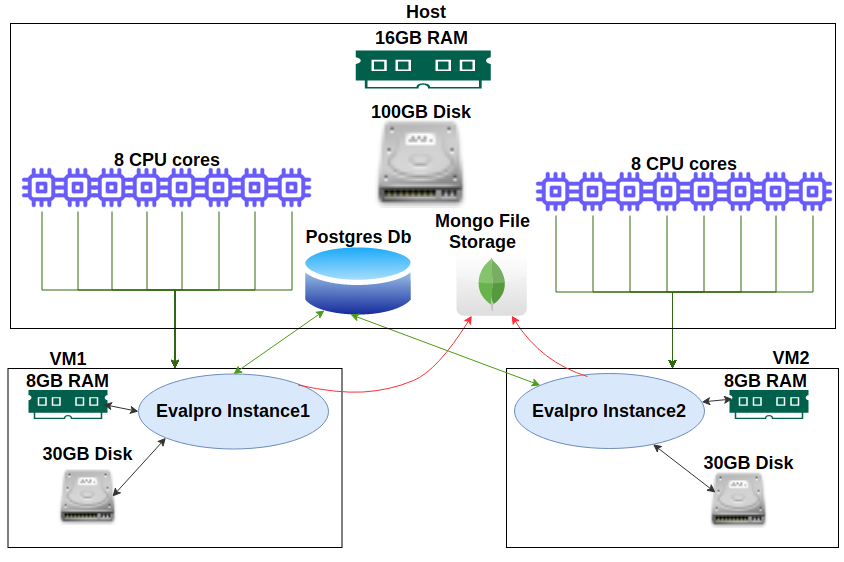
\includegraphics[scale=0.45]{Images/shared_vm_mongo.png}
  \caption{User data and Files sharing VM setup with  MongoDB}
  \label{shared_vm_mongo}
\end{figure}


\begin{table}[!htb]
    \centering
  \begin{tabularx}{\textwidth}{|X|X|X|}
    \hline
    &\makecell{Baseline}&\makecell{Data and Files sharing \\VM setup with MongoDB}\\
    \hline
    \makecell{$Throughput_{max}(1)$\\(req/sec)} & \makecell{0.3} & \makecell{0.29}\\
    \hline
    \makecell{$Throughput_{max}(16)$\\(req/sec)} & \makecell{3.37} & \makecell{3.5}\\
    \hline
    \makecell{Ideal $Throughput_{max}(1)$\\(req/sec)} & \makecell{4.8} & \makecell{4.64}\\
    \hline
    \makecell{$S(16)$} & \makecell{11.23} & \makecell{12}\\
  \hline
\end{tabularx}
\caption{Baseline vs User data and Files sharing VM setup with  MongoDB}
  \label{tab:baseline_mongo_comparision}
\end{table}




Even though the improvement in  $Throughput_{max}(16)$ and $S(16)$  we observed is very low using User data and Files sharing VM setup with  MongoDB setup, shown in the figure \ref{shared_vm_mongo}. we hypothesize that when the number of CPU cores, $N$ is high i.e 64 cores, then using User data and Files sharing VM setup with MongoDB will significantly improve the throughput, $Throughput_{max}(N)$ and the scalability factor, $S(N)$ compared to the baseline values of the throughput and the scalability factor respectively . We performed experiments using a server machine with 64 CPU cores to validate this hypothesis. The coming chapter briefly describes these experiments.

\chapter{Experiments on 64 CPU Cores Server}\label{exp_64}
We hypothesised at the end of previous chapter that when the number of CPU cores, $N$ is high i.e 64 cores, then using the User data and Files sharing VM setup with MongoDB will significantly improve the throughput, $Throughput_{max}(N)$ and the scalability factor, $S(N)$ compared to the baseline values of the throughput and the scalability factor, respectively. Therefore  to validate this hypothesis, in this chapter we performed experiments on the 64 CPU core server.  The section \ref{baseline_64} discusses about the baseline experiments using 64 CPU core server shown in the table \ref{tab:hardware_64_cores}. In the section \ref{mongo_64_cores},  we perform experiments with the User data and Files sharing VM setup with MongoDB on the 64 CPU core server and compare these results with the baseline results. Even though we mentioned in the section \ref{isolated_setup_16} that using the Completely Isolated VM setup shown in the figure \ref{isolated_vm} is very complex and infeasible approach for the scalability. In the section \ref{isolated_64_cores}, we performed experiments using the 64 CPU core server with the Completely Isolated VM setup, to see whether using 64 CPU cores still improves the throughput and the scalability factor compared to the baseline values.

\section{Baseline - 64}\label{baseline_64}
As shown in the table \ref{tab:hardware_64_cores}, the server on which the Evalpro application is running now has 64 CPU cores. Using which we have performed the baseline experiments on the Evalpro architecture shown in the figure \ref{fig:evalpro_arch}, with the user session shown in the figure \ref{user_session}. As shown in the figure \ref{baseline_64_setup}, we used a single WSGI+Celery replica and performed experiments by altering the number of CPU cores available. The observed throughput is the throughput we observed from our experiments. The ideal throughput with $N$ CPU cores is the desired throughput which is equal to $N*Throughput_{max}(1)$. The observed value of $Throughput_{max}(1)$ is 0.66 requests per second.

\begin{table}[!htb]
  \begin{tabular}{|c|p{9em}|c|c|c|c|c|}
    \hline
    Type&CPU&Cores&Memory&L3 Cache&L2 cache&L1 cache\\
    \hline
    Server & Intel\textsuperscript{R} Xeon\textsuperscript{R} CPU E5-2683 v4 @ 2.10GHz& 64&128GB&80MB&8MB&1MB\\
    \hline
    Client & AMD Opteron\textsuperscript{TM} Processor 6212 & 16&16GB&6MB&2MB&64KB\\
    \hline
    Client & AMD Opteron\textsuperscript{TM} Processor 6278 & 16&16GB&6MB&2MB&64KB\\
    \hline
    Client & Intel\textsuperscript{R} Xeon\textsuperscript{R} CPU E5-2650 v2 @ 2.60GHz & 16&16GB&20MB&256KB&32KB\\
  \hline
\end{tabular}
\caption{Hardware specifications for  Baseline-64 Experiments}
  \label{tab:hardware_64_cores}
\end{table}



\begin{figure}[!htb]
  \centering
  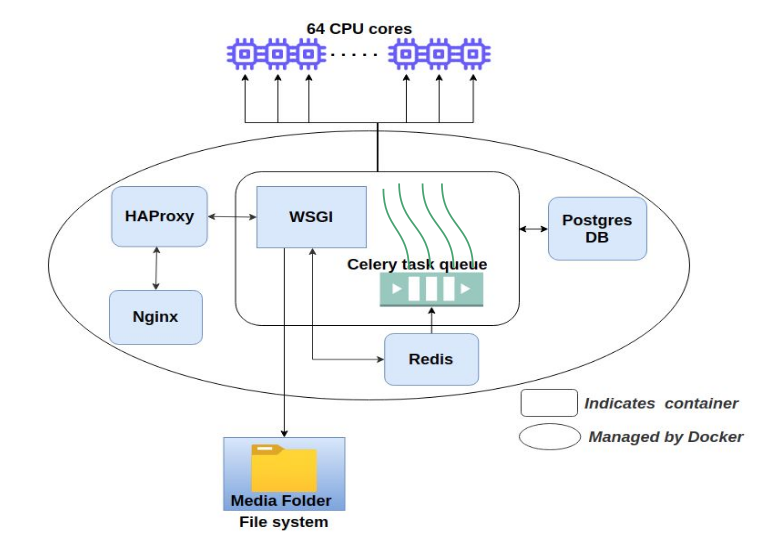
\includegraphics[width=\linewidth]{Images/Baseline-64.png}
  \caption{Baseline-64 experiment setup}
  \label{baseline_64_setup}
\end{figure}


As shown in the figure \ref{baseline_throughput_64_cores}, when the number of CPU cores $N$ increases, the maximum throughput achieved with $N$ CPU cores, $Throughput_{max}(N)$ increases. But when the number of CPU cores $N>16$, the difference between the  observed and the ideal values of $Throughput_{max}(N)$ is significantly high , i.e., throughput is not scaling linearly.

\begin{figure}[!htb]
  \centering
  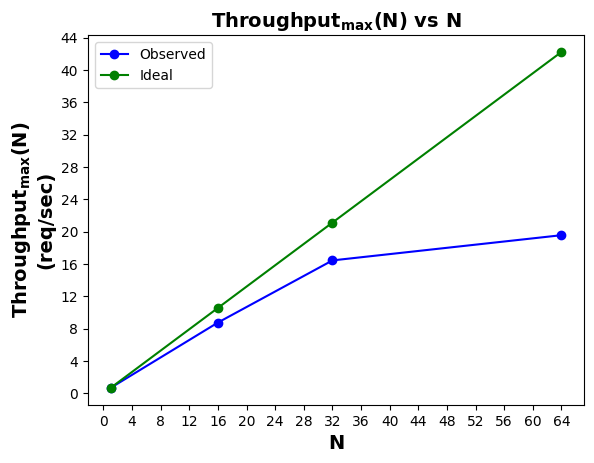
\includegraphics[width=\linewidth]{Images/Baseline-64_throughput.png}
  \caption{Baseline throughput plot with 64 CPU cores}
  \label{baseline_throughput_64_cores}
\end{figure}

To measure the scaling of throughput, we calculated the scalability factor with $N$ CPU cores, $S(N)$ using the equation \ref{eq:1}. Using the figure \ref{baseline_scalability_64_cores}, we have compared the observed scalability factor with the ideal scalability factor. The observed scalability factor for 64 CPU cores is 29.6, but the ideal  S(64) value is 64, which is shown in the table \ref{tab:baseline_64_results}. These results show that our Evalpro application is not scaling proportionally with the baseline setup having 64 CPU core server. Moreover, when the throughput achieved is maximum, the CPU utilization of the server is around 90-100\%. By this, we concluded that there are no application bottlenecks. 




\begin{figure}[!htb]
  \centering
  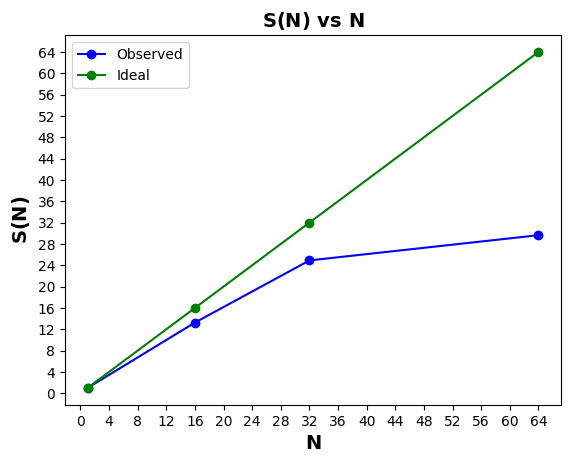
\includegraphics[width=\linewidth]{Images/Baseline-64_scalability.png}
  \caption{Baseline  Throughput Scalability plot with 64 CPU cores}
  \label{baseline_scalability_64_cores}
\end{figure}

\begin{table}[!htb]
    \centering
  \begin{tabularx}{\textwidth}{|X|X|}
    \hline
    \makecell{$Throughput_{max}(1)$ \\ (req/sec)} & \makecell{0.66}\\
    \hline
    \makecell{$Throughput_{max}(16)$ \\ (req/sec)} & \makecell{8.75}\\
    \hline
    \makecell{$Throughput_{max}(32)$ \\ (req/sec)} & \makecell{16.44}\\
    \hline
    \makecell{$Throughput_{max}(64)$ \\ (req/sec)} & \makecell{19.56}\\
    \hline
    \makecell{Ideal $Throughput_{max}(64)$ \\ (req/sec)} & \makecell{42}\\
    \hline
    \makecell{$S(16)$} & \makecell{13.25}\\
    \hline
    \makecell{$S(32)$} & \makecell{25}\\
    \hline
    \makecell{$S(64)$} & \makecell{29.6}\\
  \hline
\end{tabularx}
\caption{Baseline - 64 Experiments results}
  \label{tab:baseline_64_results}
\end{table}







Based on our hypothesis at the end of previous chapter that when the number of CPU cores, $N$ is high i.e 64 cores, then using the User data and Files sharing VM setup with MongoDB will significantly improve the throughput, $Throughput_{max}(N)$ and the scalability factor, $S(N)$ compared to the baseline values of the throughput and the scalability factor respectively. Therefore to see the improvement in both  $S(N)$ and $Throughput_{max}(N)$, when the number of CPU cores $N>16$, we performed experiments using the User data and Files sharing VM setup with MongoDB on 64 CPU cores, shown in the figure \ref{shared_vm_mongo_64_cores}. The next section briefly describes these experiments.

\section{MongoDB for File Storage - 64}\label{mongo_64_cores}
In this section we validate our hypothesis that when the number of CPU cores, $N$ is high i.e 64 CPU cores, then using the User data and Files sharing VM setup with MongoDB will significantly improve the throughput, $Throughput_{max}(N)$ and the scalability factor, $S(N)$ compared to the baseline values of the throughput and the scalability factor respectively. Therefore the experiments described in the chapter \ref{mongodb_filestorage} are performed on the new server machine having 64 CPU cores, shown in the table \ref{tab:hardware_64_cores}. As shown in the figure \ref{shared_vm_mongo_64_cores},  we have created 4 VMs using KVM-QEMU, with each VM assigned 16 different CPU cores, 32GB RAM, and 100GB hard disk, and the Evalpro application instance is run on each VM. All the 4 VMs are sharing the MongoDB running on the host.


\begin{figure}[!htb]
  \centering
  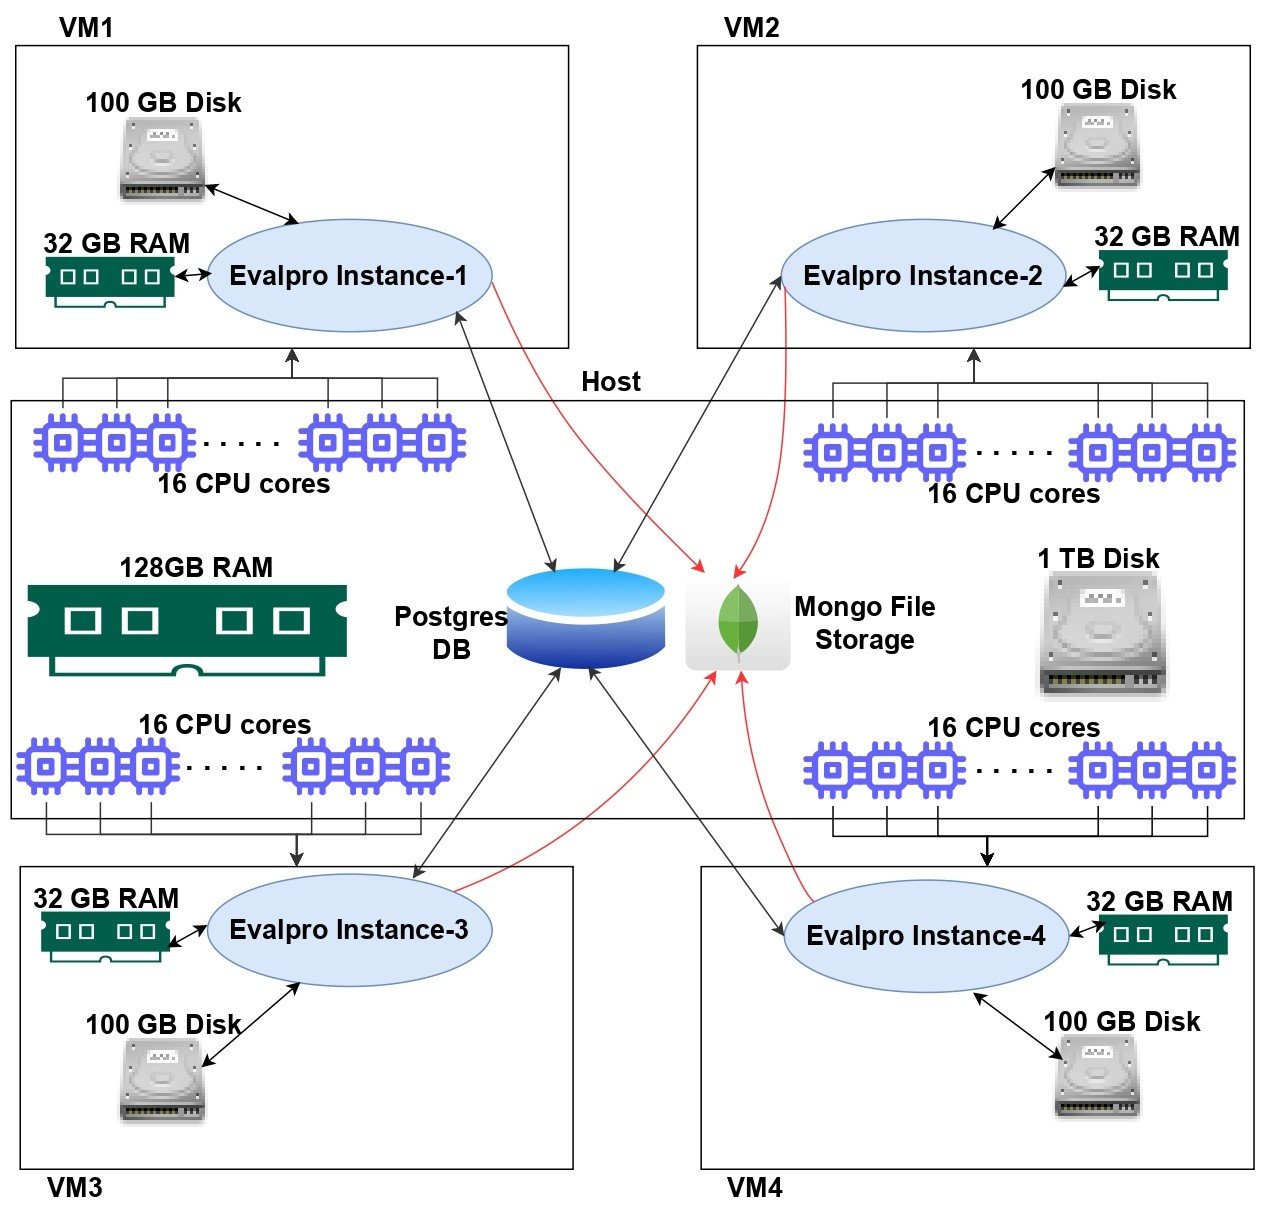
\includegraphics[width=\linewidth]{Images/shared_vm_mongo_64_cores.png}
  \caption{User data and Files sharing VM setup with  MongoDB (64 CPU cores)}
  \label{shared_vm_mongo_64_cores}
\end{figure}

Using the user session shown in the figure \ref{user_session}, we have performed experiments with the new Evalpro architecture which uses MongoDB for file storage, shown in the figure \ref{architecture_mongo}. The maximum throughput achieved on the single CPU core, $Throughput_{max}(1)$ was observed to be 0.47 requests per second. We performed experiments using the User data and Files sharing VM setup with MongoDB, shown in the figure \ref{shared_vm_mongo_64_cores}. We found that the maximum throughput achieved on the 64 CPU cores, $Throughput_{max}(64)$ to be 11.27 requests per second. We calculated $S(64)$, the scalability factor with 64 CPU cores using the equation \ref{eq:1}, by which the $S(64)$ value is 24. We compared the values of $Throughput_{max}(64)$ and $S(64)$ with the baseline results. As shown in the table \ref{tab:baseline_shared_vm_mongo_64_cores}, both the maximum throughput achieved on the 64 CPU cores, $Throughput_{max}(64)$ and the scalability factor with 64 CPU cores, $S(64)$ is lower than the baseline values of 19.56 requests per second and 29.6, respectively.



\begin{table}[!htb]
    \centering
  \begin{tabularx}{\textwidth}{|X|X|X|}
    \hline
    &\makecell{Baseline - 64}&\makecell{Data and Files sharing \\VM setup with MongoDB\\(64 CPU cores)}\\
    \hline
    \makecell{$Throughput_{max}(1)$\\(req/sec)} & \makecell{0.66} & \makecell{0.47}\\
    \hline
    \makecell{$Throughput_{max}(64)$\\(req/sec)} & \makecell{19.56} & \makecell {11.27}\\
    \hline
    \makecell{Ideal $Throughput_{max}(1)$\\(req/sec)} &\makecell{42} & \makecell{30}\\
    \hline
    \makecell{$S(64)$} & \makecell{29.6} & \makecell{24}\\
  \hline
\end{tabularx}
\caption{Baseline - 64 vs User data and Files sharing VM setup with  MongoDB \\\tab\tab\tab\tab\tab\tab(64 CPU cores)}
  \label{tab:baseline_shared_vm_mongo_64_cores}
\end{table}





By the above results, we came to conclusion that our hypothesis, when the number of CPU cores, $N$ is high i.e 64 cores, the value of  $Throughput_{max}(N)$ and $S(N)$ using MongoDB, with the shared VM experiment setup will be significantly higher than the baseline  $Throughput_{max}(N)$ and $S(N)$ values, respectively, is wrong.

Even though it is mentioned in the section \ref{isolated_setup_16} that the Completely Isolated VM setup is very complex and infeasible approach for the scalability. We tried to find whether using the Completely Isolated VM setup, shown in the figure \ref{isolated_vm_64_cores}, with 64 CPU cores server improves the throughput scalability of the Evalpro application. The next section briefly describes about these experiments.


\section{Completely Isolated VM setup - 64}\label{isolated_64_cores}

In this section we performed experiments on the 64 CPU core server with the Completely Isolated VM setup, to see whether using 64 CPU cores still improves the  throughput and the scalability factor compared to the baseline values of the Evalpro application. Therefore the experiments described in the section \ref{isolated_setup_16} are performed on the new server machine having 64 CPU cores, shown in the table \ref{tab:hardware_64_cores}. As shown in the figure \ref{isolated_vm_64_cores},  we have created 4 VMs using KVM-QEMU, with each VM assigned 16 different CPU cores, 32GB RAM, and 100GB hard disk, and the Evalpro application instance is run on each VM. All the 4 VMs are run in a completely isolated manner.


\begin{figure}[!htb]
  \centering
  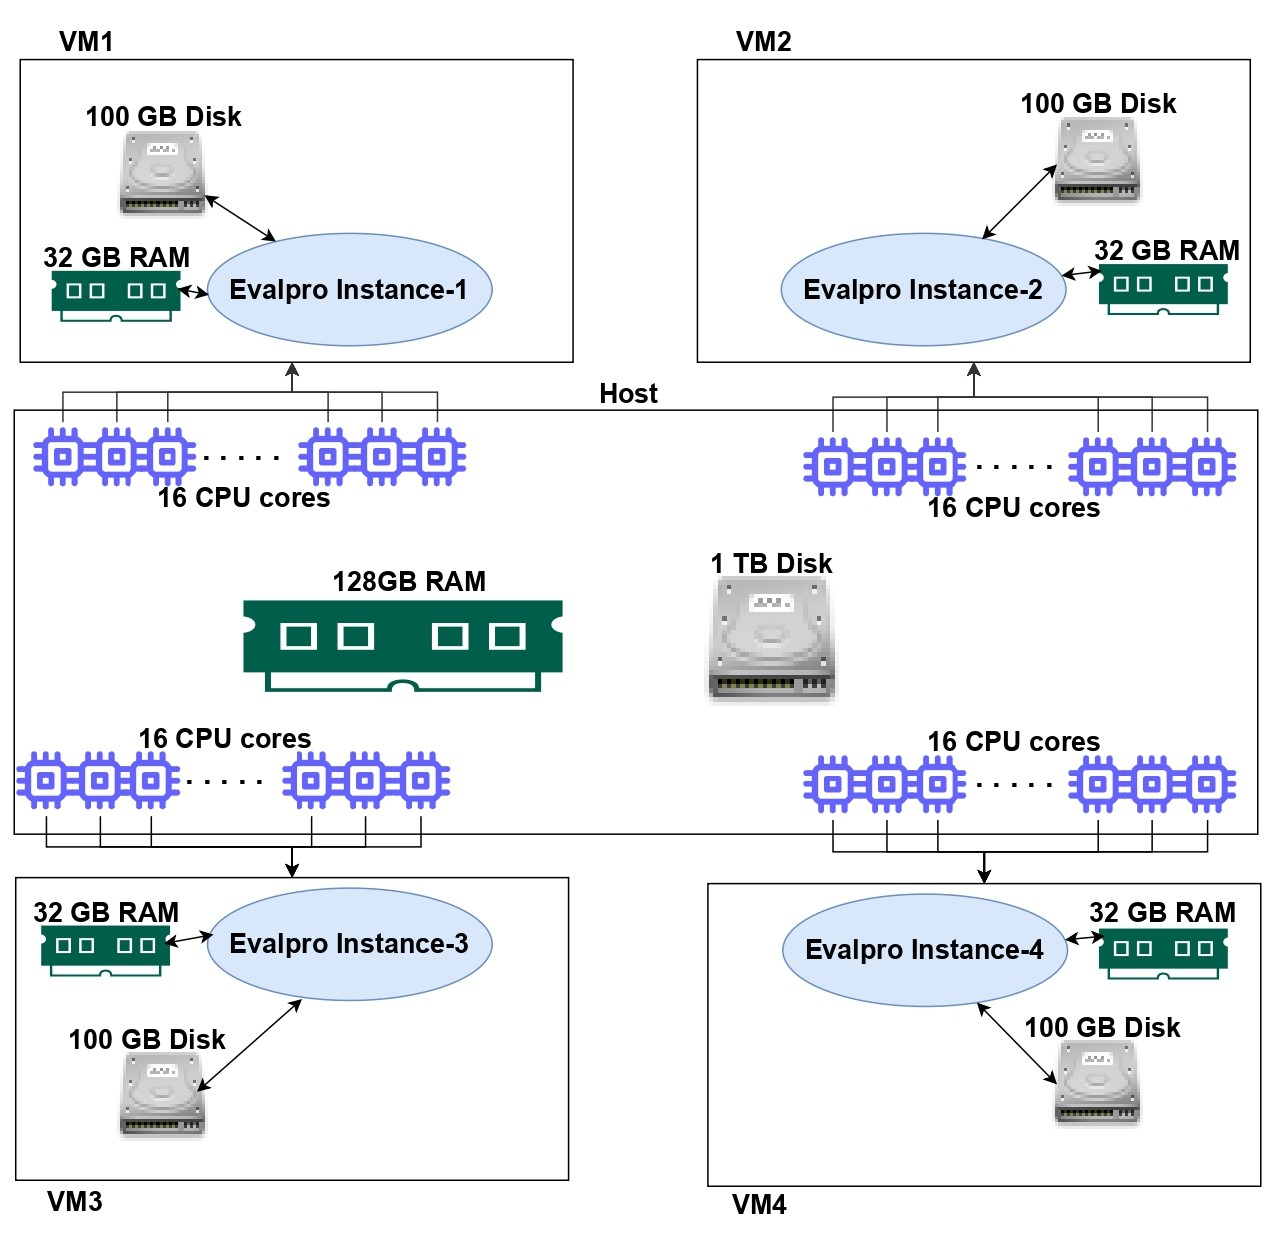
\includegraphics[width=\linewidth]{Images/isolated-vm-64.jpg}
  \caption{Completely Isolated VM setup (64 CPU cores)}
  \label{isolated_vm_64_cores}
\end{figure}

Using the user session shown in the figure \ref{user_session}, we have performed experiments with the current Evalpro architecture shown in the figure \ref{fig:evalpro_arch}. The maximum throughput achieved on the single CPU core, $Throughput_{max}(1)$ was observed to be 0.66 requests per second. We performed experiments using the  Isolated VM setup shown in the figure \ref{isolated_vm_64_cores}. We found that the maximum throughput achieved on the 64 CPU cores, $Throughput_{max}(64)$ to be 15.03 requests per second. We calculated $S(64)$, the scalability factor with 64 CPU cores using the equation \ref{eq:1}, by which the $S(64)$ value is 23. We compared the values of $Throughput_{max}(64)$ and $S(64)$ with the baseline results. As shown in the table \ref{tab:baseline_isolated_64_cores}, both the maximum throughput achieved on the 64 CPU cores, $Throughput_{max}(64)$ and the scalability factor with 64 CPU cores, $S(64)$ is lower than the baseline values of 19.56 requests per second and 29.6, respectively. By these results, we came to the conclusion that by using 64 CPU core server with Completely isolated VM setup doesn't improve the throughput scalability of the Evalpro application



\begin{table}[!htb]
    \centering
  \begin{tabularx}{\textwidth}{|X|X|X|}
    \hline
    &\makecell{Baseline - 64}&\makecell{Completely Isolated \\ VM setup - 64}\\
    \hline
    \makecell{$Throughput_{max}(1)$\\(req/sec)} & \makecell{0.66} & \makecell{0.66}\\
    \hline
    \makecell{$Throughput_{max}(64)$\\(req/sec)} & \makecell{19.56} & \makecell{15.03}\\
    \hline
    \makecell{Ideal $Throughput_{max}(1)$\\(req/sec)} & \makecell{42} & \makecell{42}\\
    \hline
    \makecell{$S(64)$} & \makecell{29.6} & \makecell{23}\\
  \hline
\end{tabularx}
\caption{Baseline - 64 vs Completely Isolated VM setup (64 CPU cores)}
  \label{tab:baseline_isolated_64_cores}
\end{table}


To find the best scalability  of the Evalpro like workload on a given platform, we have developed micro benchmarks, which depict whether the limitation in the scalability is due to the workload or inherent to the platform. The next chapter briefly describes about the micro-benchmark experiments.

\chapter{Micro benchmark Experiments}\label{micro_benchmark_exps}
Micro benchmarks are simple, lightweight, portable benchmarks for establishing the best
scalability of the workload for a given platform, which are used to isolate whether scalability limit is due to the workload, or inherent to the platform. We have developed two different types of micro benchmarks i.e CPU micro benchmark and Evalpro micro benchmark. The coming sections briefly describe about them.
\section{CPU micro benchmark}
To find the best scalability we can get for a raw CPU workload, a completely CPU bound benchmark is created with consists a tight loop of 200 iterations, each iteration runs the CPU bound job, which increments a counter in the loop for large number  of iterations i.e 100000000. The CPU micro benchmark is run on the server having 64 CPU cores shown in the table \ref{tab:hardware_64_cores}. 

\begin{figure}[!htb]
  \centering
  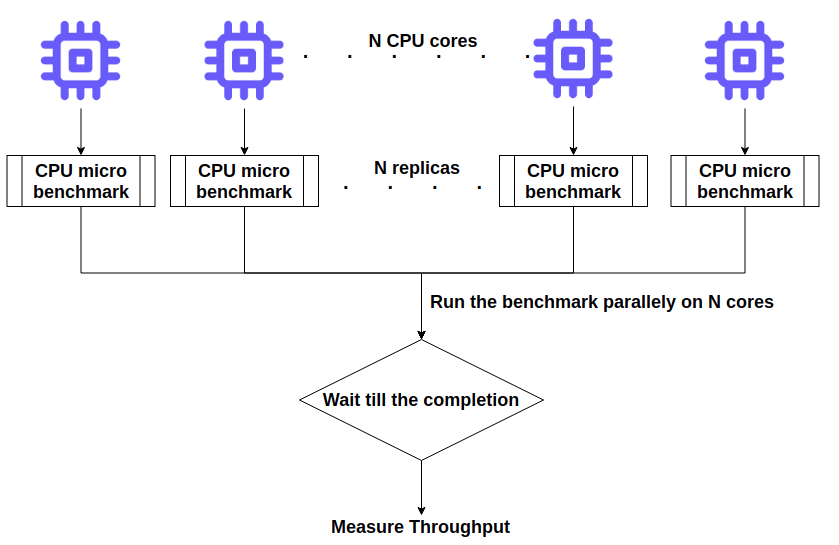
\includegraphics[width=\linewidth]{Images/cpu_micro_benchmark.png}
  \caption{CPU micro benchmark experiment setup}
  \label{cpu_micro_bench_mark}
\end{figure}

As shown in the figure \ref{cpu_micro_bench_mark}, we have pinned each replica of CPU micro benchmark to a CPU core using Linux taskset command. By altering the value of $N$, the number of CPU cores available, between 1 to 64, we have run $N$ replicas parallely on $N$ CPU cores and measured the throughput, since all the $N$ CPU cores are completely utilized the throughput we measured is the maximum throughput $Throughput_{max}(N)$

The figure \ref{cpu_micro_bench_mark_throughput}, shows that, when the number of CPU cores $N$ increases, the observed throughput, $Throughput_{max}(N)$ increases. But when the number of CPU cores $N>32$, then the difference between the values of the observed  $Throughput_{max}(N)$  and the ideal $Throughput_{max}(N)$ is slightly high. To measure the scaling of throughput, we calculated the scalability factor with $N$ CPU cores, $S(N)$ using the equation \ref{eq:1}. Using the figure \ref{cpu_micro_bench_mark_scalability}, we have compared the observed scalability factor with the ideal scalability factor. The observed scalability factor  for 64 CPU cores is 48, but the ideal  S(64) value is 64. By these results we came to the conclusion the even for a raw CPU micro benchmark 48 is the best scalability factor we can get with 64 CPU cores.


\begin{figure}[!htb]
  \centering
  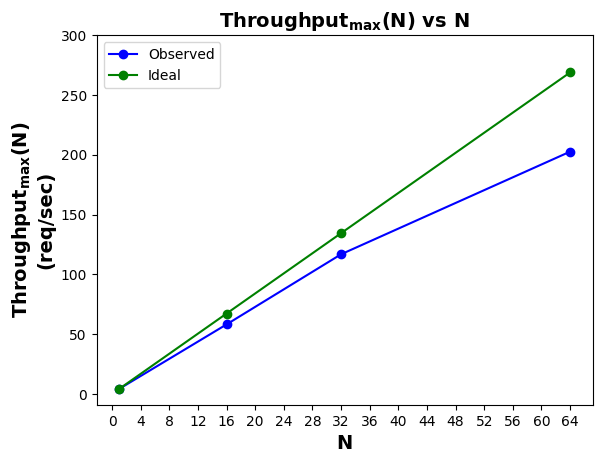
\includegraphics[width=\linewidth]{Images/cpu_micro_benchmark_throughput.png}  \caption{CPU micro benchmark throughput plot}
  \label{cpu_micro_bench_mark_throughput}
\end{figure}

\begin{figure}[!htb]
  \centering
  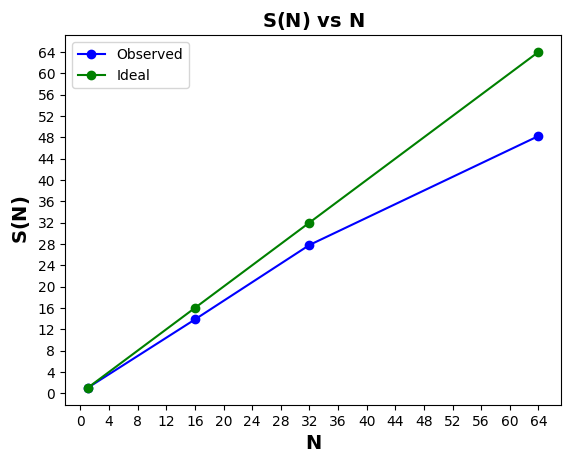
\includegraphics[width=\linewidth]{Images/cpu_micro_benchmark_scalability.png}
  \caption{CPU micro benchmark throughput scalability plot}
  \label{cpu_micro_bench_mark_scalability}
\end{figure}

\section{Evalpro micro benchmark}\label{evalpro_micro_benchmark_section}
To find the reason for scalability limitation shown in the section \ref{baseline_64} of Evalpro application, we designed a Evalpro micro benchmark because the micro benchmark has few lines of code, it will be easier to perform low level bottleneck analysis on it  compared to the entire application. The  Evalpro micro benchmark runs the auto-grading session i.e compilation of the code, execution of the object code generated by compilation and comparing the expected output with  the actual output. For compilation we used g++ compiler. The auto-grading session is run in a tight loop of 75 iterations. The Evalpro micro benchmark is run on the server having 64 CPU cores shown in the table \ref{tab:hardware_64_cores}.
\begin{figure}[!htb]
  \centering
  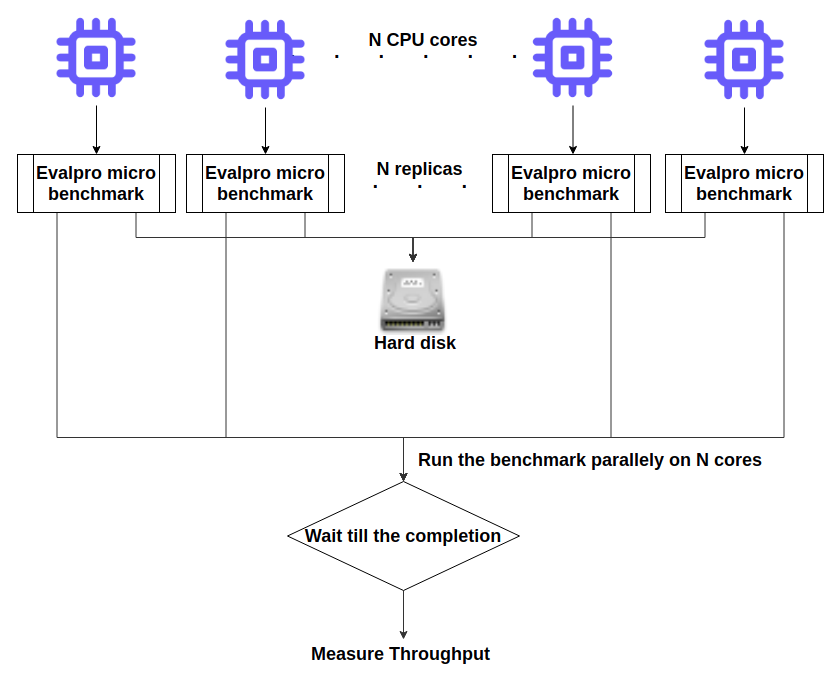
\includegraphics[width=\linewidth]{Images/evalpro_micro_benchmark.png}
  \caption{Evalpro micro benchmark experiment setup}
  \label{evalpro_micro_bench_mark}
 
\end{figure}

As shown in the figure \ref{cpu_micro_bench_mark}, we have pinned each replica of Evalpro micro benchmark to a CPU core using Linux taskset command and all the Evalpro micro benchmark replicas use the hard disk to read and write files while running the Evalpro auto-grader session. By altering the value of $N$, the number of CPU cores available, between 1 to 64, we have run $N$ replicas parallely on $N$ CPU cores and measured the throughput, since all the $N$ CPU cores are completely utilized the throughput we measured is the maximum throughput,  $Throughput_{max}(N)$

\begin{figure}[!htb]
  \centering
  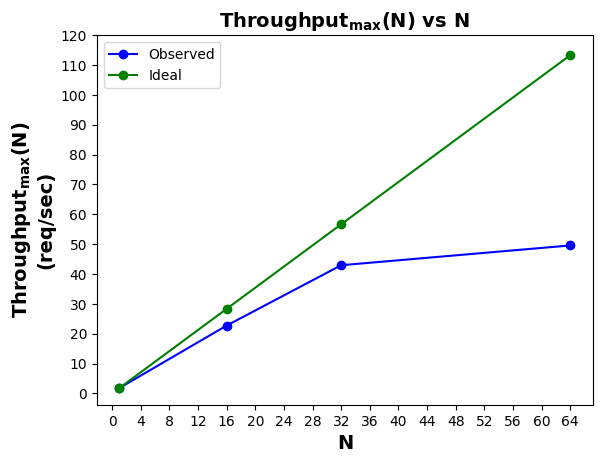
\includegraphics[scale=0.9]{Images/evalpro_micro_benchmark_throughput.png}
  \caption{Evalpro micro benchmark throughput plot}
  \label{evalpro_micro_bench_mark_throughput}
 
\end{figure}

The figure \ref{evalpro_micro_bench_mark_throughput}, shows that, when the number of CPU cores $N$ increases, the observed throughput, $Throughput_{max}(N)$ increases. But when the number of CPU cores $N>16$, then the difference between the values of the observed  $Throughput_{max}(N)$  and the ideal $Throughput_{max}(N)$ is much higher than the difference observed for the CPU micro benchmark shown in the figure \ref{cpu_micro_bench_mark_throughput}. To measure the scaling of throughput, we calculated the scalability factor with $N$ CPU cores, $S(N)$ using the equation \ref{eq:1}.  Using the figure \ref{evalpro_micro_bench_mark_scalability}, we have compared the observed scalability factor with the ideal scalability factor. The scalability factor we got for 64 CPU cores is 28, but the ideal  S(64) value is 64.


\begin{figure}[!htb]
  \centering
  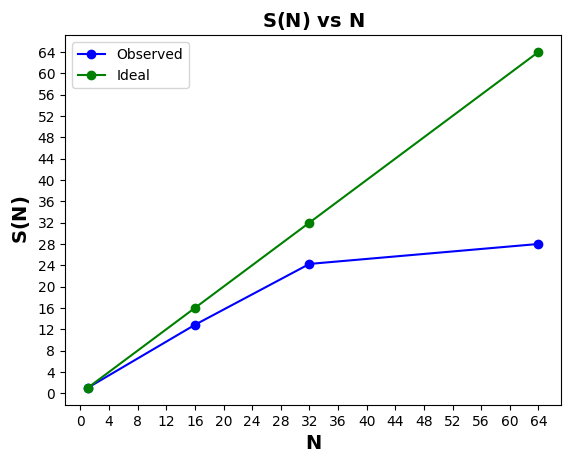
\includegraphics[scale=0.9]{Images/evalpro_micro_benchmark_scalability.png}
  \caption{Evalpro micro benchmark throughput scalability plot}
  \label{evalpro_micro_bench_mark_scalability}
 
\end{figure}

\begin{figure}[!htb]
  \centering
  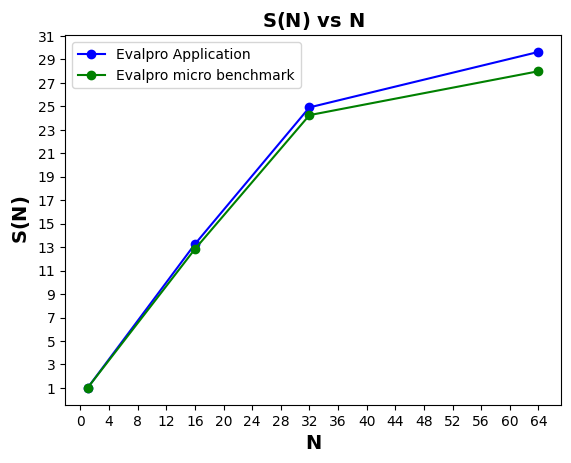
\includegraphics[width=\linewidth]{Images/scalability_comparision.png}
  \caption{Throughput Scalability of Evalpro Application vs Evalpro micro benchmark}
  \label{evalpro_scalability_comparision}
\end{figure}


We have compared the Evalpro application's  baseline scalability factor calculated in section \ref{baseline_64} with the Evalpro micro benchmark's scalability factor calculated above. As shown in the figure \ref{evalpro_scalability_comparision}, Evalpro application and micro benchmark scalability factor $S(N)$ values are very close. Since  the scalability factor of Evalpro application and Evalpro micro benchmark are almost same, therefore we hypothesise that the reason for scalability limitation of Evalpro application will be same as the reason for Evalpro micro benchmark. Therefore we have performed bottleneck analysis on the Evalpro micro benchmark to find the reason for its scalability limitation. The next chapter briefly describes about bottleneck analysis on the Evalpro micro benchmark.



\chapter{Micro benchmark Bottleneck Analysis}\label{micro_benchmark_bottleneck_analysis}

For Evalpro micro benchmark, we observed  limitation in the scalability factor $S(N)$ for $N>16$ in the previous section. We performed the low level bottleneck analysis on the Evalpro micro benchmark to find the reason for its scalability limitation. Moreover since the micro benchmark has few lines of code, it will be easier to perform low level bottleneck analysis on the micro benchmark compared to the entire application. In this section we have performed low level bottleneck analysis on the Evalpro micro benchmark.

\section{Using Tmpfs in place of Hard Disk}
Tmpfs \cite{tmpfs} is an in-memory file system which stores file in the memory instead of disk. We hypothesised that the usage of disk by multiple Evalpro micro benchmark replicas, as shown in the figure \ref{evalpro_micro_bench_mark}, is limiting its scalability factor $S(N)$ for $N>16$. So, as shown in the figure \ref{evalpro_micro_benchmark_tmpfs}, we used Tmpfs instead of hard disk to store,read files while running Evalpro auto-grading session
\begin{figure}[!htb]
  \centering
  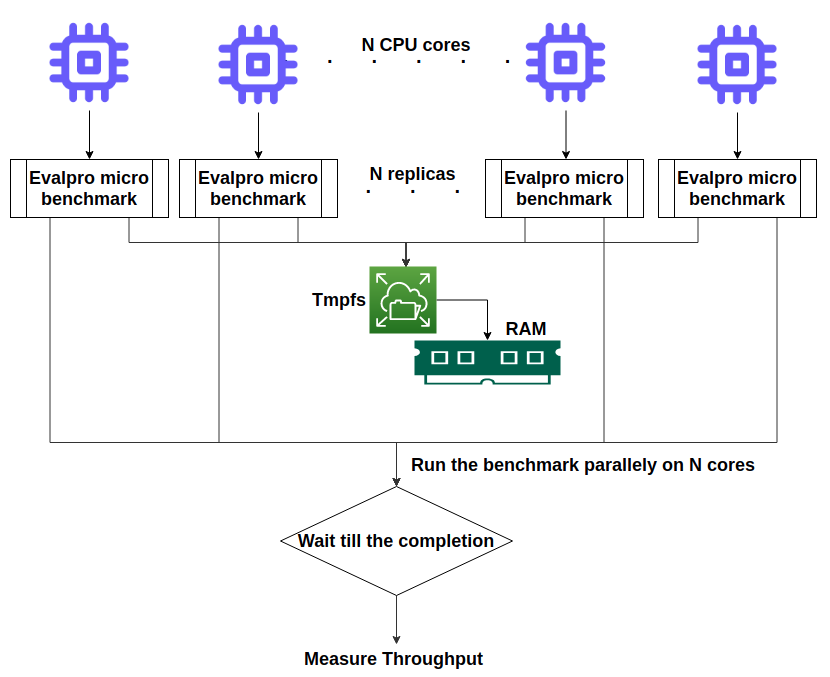
\includegraphics[width=\linewidth]{Images/evalpro_micro_benchmatk_tmpfs.png}
  \caption{ Evalpro micro benchmark using Tmpfs}
  \label{evalpro_micro_benchmark_tmpfs}
\end{figure}


The throughput we measured using Tmpfs with $N$ CPU cores, $Throughput_{max}(N)$ is compared with $Throughput_{max}(N)$ using Hard disk. From the figure \ref{evalpro_micro_benchmark_tmpfs_comparision}, it is clear that using Tmpfs in place of hard disk to store,read files  makes no significant difference in the throughput. Thus we came to the conclusion that using disk to store,read files while running Evalpro auto-grader session is not the bottleneck i.e not the reason for limitation in the scalability.

\begin{figure}[!htb]
  \centering
  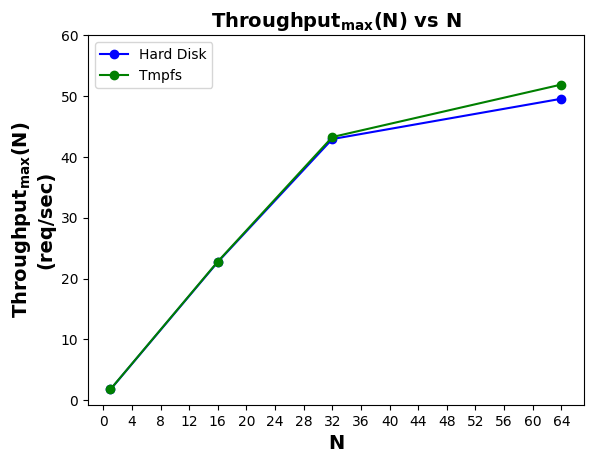
\includegraphics[width=\linewidth]{Images/hard_disk_tmpfs_comparision.png}
  \caption{ Comparison of Tmpfs and Hard disk}
  \label{evalpro_micro_benchmark_tmpfs_comparision}
\end{figure}

\section{Low level bottleneck analysis using PERF}\label{low_level_bottleneck_analysis}

PERF \cite{PERF} tool  is used to closely monitor a workload to get information about different types of software, hardware events raised during the execution of the workload. We used  PERF tool to count the occurrence of the following events during the execution of the Evalpro micro benchmark.
\begin{itemize}
\item {\texttt{LLC-loads}}: counts the number of memory accesses which load data from the  Last level cache  i.e L3 cache.
 \item {\texttt{LLC-load-misses}}: counts the number of memory accesses which resulted in cache miss while trying load  the data from Last level cache  i.e L3 cache.
\item {\texttt{LLC-stores}}:  counts the number of memory accesses which store data into the  Last level cache  i.e L3 cache 
\item {\texttt{LLC-store-misses}}: counts the number of memory accesses which resulted in cache miss while trying to store  the data into the Last level cache  i.e L3 cache.
\item {\texttt{page-faults}}: counts the number of memory accesses which resulted in page faults.
\item {\texttt{instructions}}: counts the number of instructions present in the workload.
\item {\texttt{branches}}: counts the number of instructions which resulted in taking the branch.
\item {\texttt{branch-misses}}: counts the number of branch instructions which the branch predictor wrongly predicted as not a branch instruction.
\end{itemize}

\begin{figure}[!htb]
  \centering
  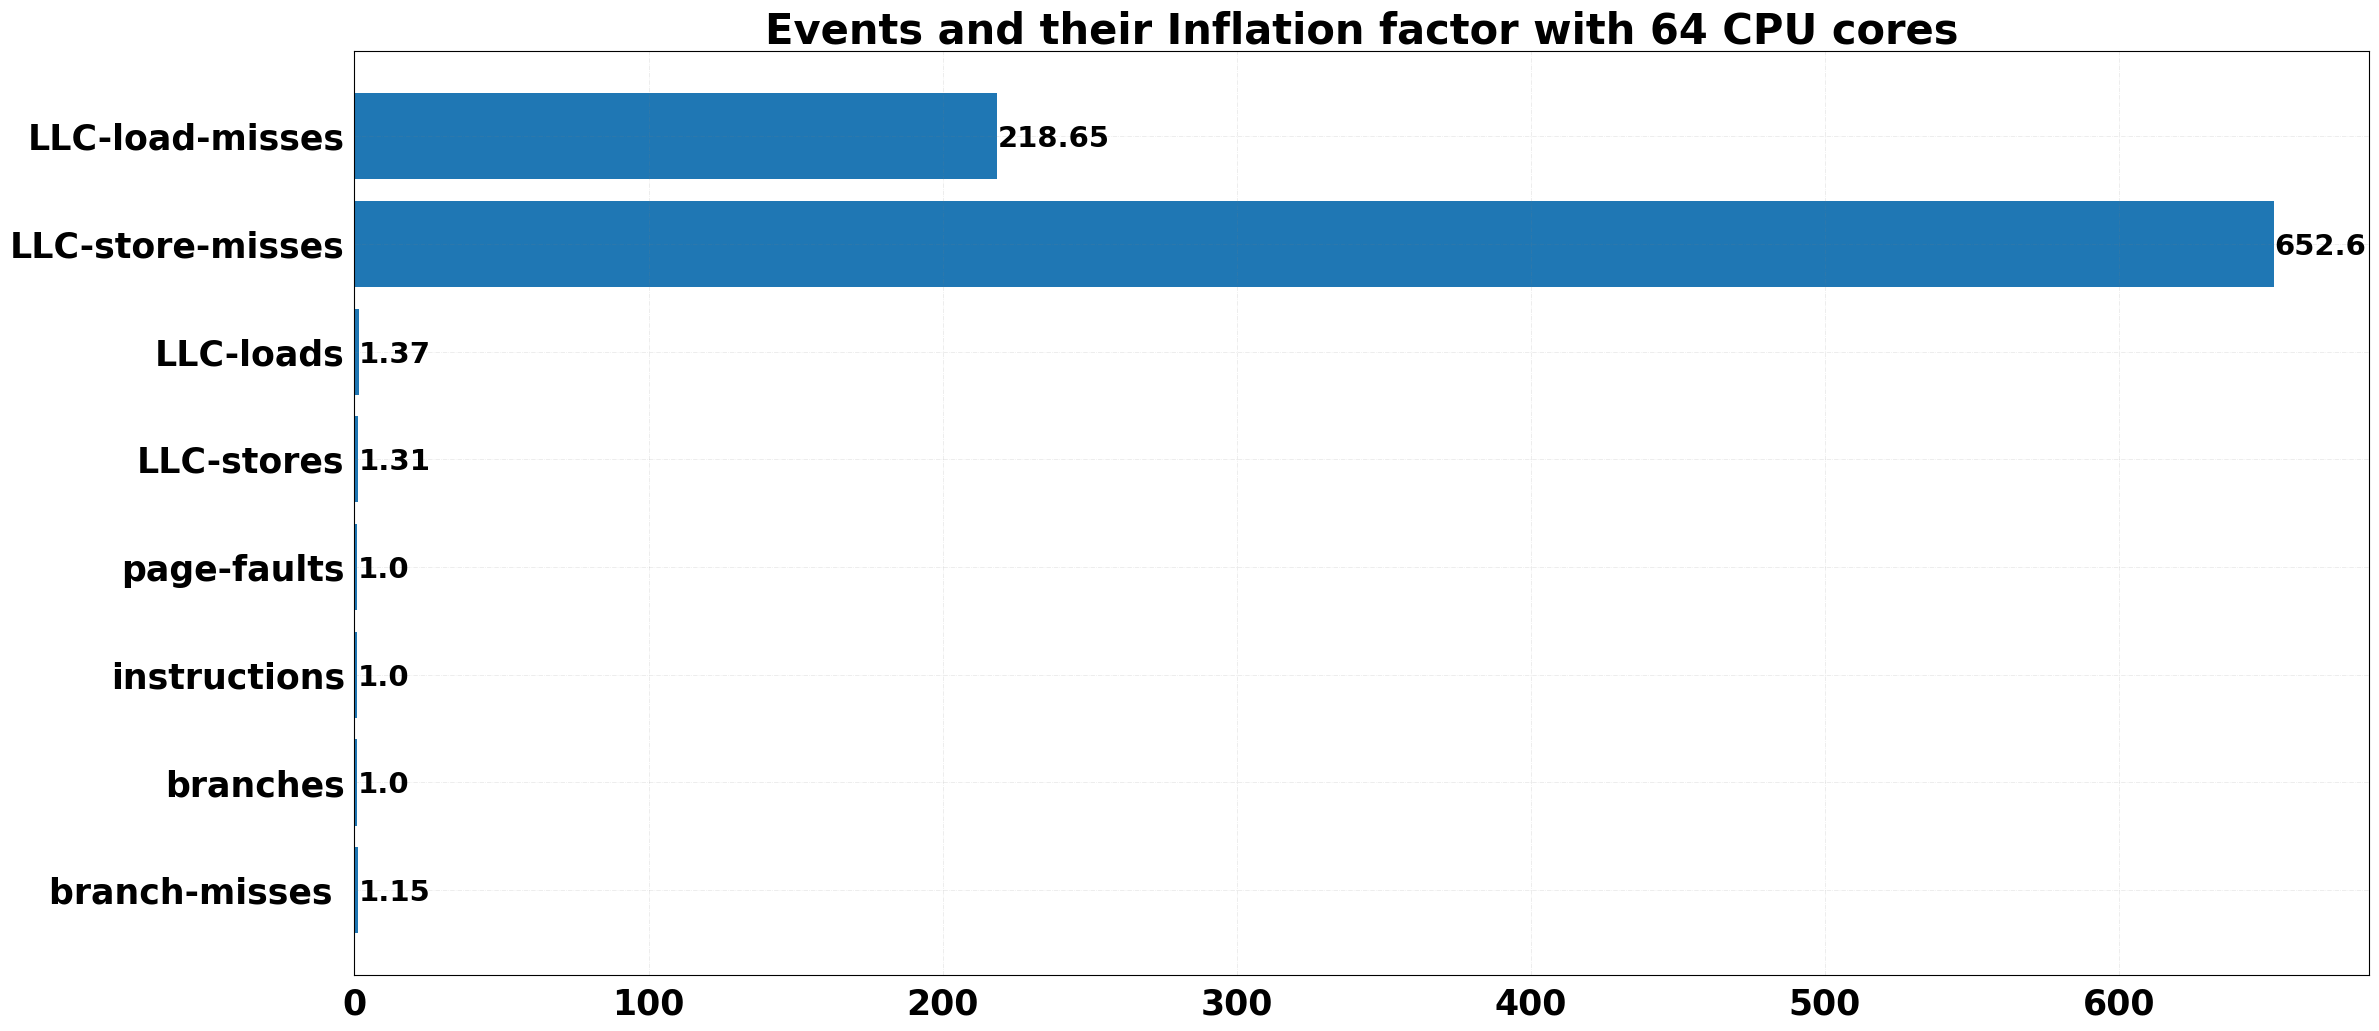
\includegraphics[width=\linewidth]{Images/perf_tool_results_final.png}
  \caption{Inflation factor of Events in Evalpro micro benchmark by Perf tool}
  \label{perf_results}
\end{figure}


 Using the PERF tool, we have measured the occurrence count of the events by running Evalpro micro benchmark with the experiment setup shown in the figure \ref{evalpro_micro_bench_mark}. We altered the number of CPU cores and number of Evalpro micro benchmark replicas, $N$ from 1 to 64. To measure the inflation in the occurrence of an event when increasing the number of CPU cores $N$, we define the Inflation factor. As shown in the equation \ref{eq:2}, for an event the Inflation factor with $N$ CPU cores is  $Inflation\_factor_{event}(N)$, which is equal to the ratio of occurrence count of the event with $N$ CPU cores normalized to a single CPU core, $Normalized\_count_{event}(N)$ and the occurrence count of the event  with a single CPU core, $Count_{event}(1)$. The Ideal value of $Inflation\_factor_{event}(N)$ is 1.

\begin{equation}
  Inflation\_factor_{event}(N)=\dfrac{Count_{event}(N)}{N \times Count_{event}(1)}=\dfrac{Normalized\_count_{event}(N)}{Count_{event}(1)}
  \label{eq:2}
\end{equation}

As shown in the figure \ref{perf_results}, the value of the  Inflation factor with 64 CPU cores, $Inflation\_factor_{event}(64)$ is very high for LLC-load-misses and LLC-store-misses. But  for other  events the value of $Inflation\_factor_{event}(64)$ is almost 1, which is negligible. By these results it is clear that LLC-load-misses and LLC-store-misses have been disproportionately inflated when the number of CPU cores $N>16$.

To find the  program in the Evalpro micro benchmark which is causing the  disproportionate inflation of LLC load and store misses, we have used PERF tool to find percentage of total LLC misses at program level. As shown the figure \ref{llc_misses_gplusplus}, it is clear that  compared to 1 CPU core, on 64 CPU cores, the percentage of total LLC misses i.e LLC-load-misses and LLC-store-misses by g++ program is very high. 

\begin{figure}[!htb]
  \centering
  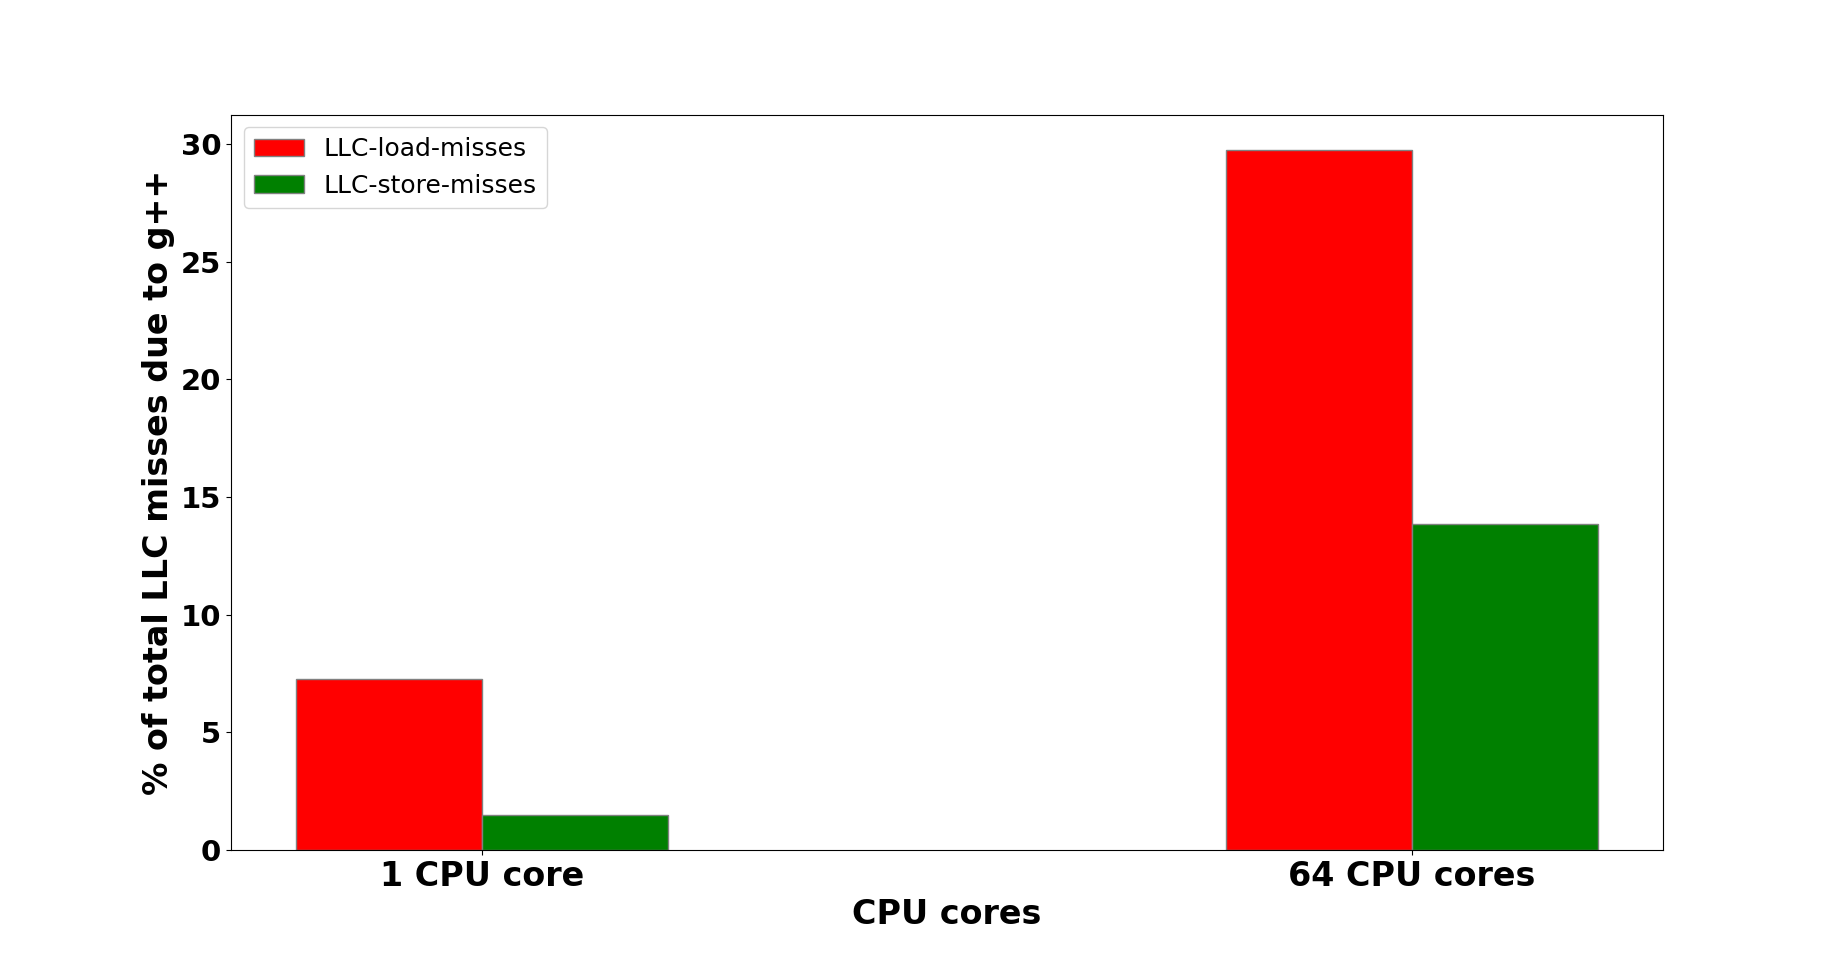
\includegraphics[width=\linewidth]{Images/llc_misses_g++.png}
  \caption{Increase in LLC misses with CPU cores by g++ }
  \label{llc_misses_gplusplus}
\end{figure}


From the above results it is clear that even though the L3 CPU cache size is 80MB,  when the L3 cache is shared with 64 Evalpro micro benchmark replicas each running on a separate CPU core then due to the memory intensive nature of g++ program, the L3 CPU cache is becoming the bottleneck. Thus the limitation in CPU cache size is the reason for scalability limitation of Evalpro micro benchmark.

Therefore we performed bottleneck analysis on the Evalpro application using the PERF, to validate our hypothesis at the end of the section \ref{evalpro_micro_benchmark_section},  that the scalability limitation of the Evalpro micro-benchmark, i.e., CPU cache, is also the reason for the scalability limitation of the Evalpro application. The following chapter briefly describes the  bottleneck analysis on the Evalpro application using the PERF tool.


\chapter{PERF analysis on the Evalpro application}\label{perf_evalpro_application}

To validate our hypothesis at the end of the section \ref{evalpro_micro_benchmark_section},  that the reason for scalability limitation of Evalpro micro benchmark  i.e  CPU cache is also the reason for scalability limitation of Evalpro application, we used the  PERF tool to count the occurrence of the different software and hardware events  raised when the load test is run on the Evalpro application.

Using the initial baseline experiment setup shown in the section \ref{baseline_16}, we used the PERF tool to monitor the occurrence count of the following events
\begin{itemize}
\item {LLC-loads}
 \item {LLC-load-misses}
\item {LLC-stores}
\item {LLC-store-misses}
\item {page-faults}
\item {instructions}
\item {branches}
\item {branch-misses}
\end{itemize}
The explanation of each event is described in the section \ref{low_level_bottleneck_analysis}. The server used for initial baseline experiments is a 16 CPU core single socket server with 20MB CPU cache (L1+L2+L3). Using equation \ref{eq:2}, we calculated inflation factor with 16 CPU cores , i.e., $Inflation\_factor_{event}(16)$. As shown in the figure \ref{perf_results_application}, the value of the  Inflation factor with 16 CPU cores, $Inflation\_factor_{event}(16)$ is significantly high for LLC-load-misses , i.e., 2.25. For LLC-store-misses it is slightly higher than 1. But  for other  events, the value of $Inflation\_factor_{event}(16)$ is less than 1. By these results, it is clear that  in our initial baseline experiments described in the section \ref{baseline_16}, LLC-load-misses have been inflated when the number of CPU cores $N>8$.

 The server machine used for final baseline experiments shown in section \ref{baseline_64} is a 64 CPU core two socket server with 89MB CPU cache (L1+L2+L3) , i.e., each socket has 32 CPU cores, 40MB L3, 8MB L2, and 1MB L1 CPU cache. The CPUs and CPU caches corresponding to the  servers used for initial and final baseline experiments belong to the same Intel\textsuperscript{R} Xeon\textsuperscript{R} Processor E5 v4  and  Intel\textsuperscript{R}  Smart Cache family, respectively.
 
For the final baseline experiments described in the section \ref{baseline_64}, in which the server has the CPU cache size of 49MB, i.e., 40MB L3, 8MB L2 , and 1MB L1 CPU cache for 16 CPU cores, we measured the occurrence count of LLC-load-misses and LLC-store-misses using the PERF tool. We have calculated the values of Inflation factor using equation \ref{eq:2}, in which for $Count_{event}(1)$, PERF event count values  measured for the initial baseline experiments with a single CPU core are used. The calculated values of $Inflation\_factor_{LLC-load-miss}(16)$ and  $Inflation\_factor_{LLC-store-miss}(16)$ values are 0.94 and 0.37 respectively. 

\begin{figure}[!htb]
  \centering
  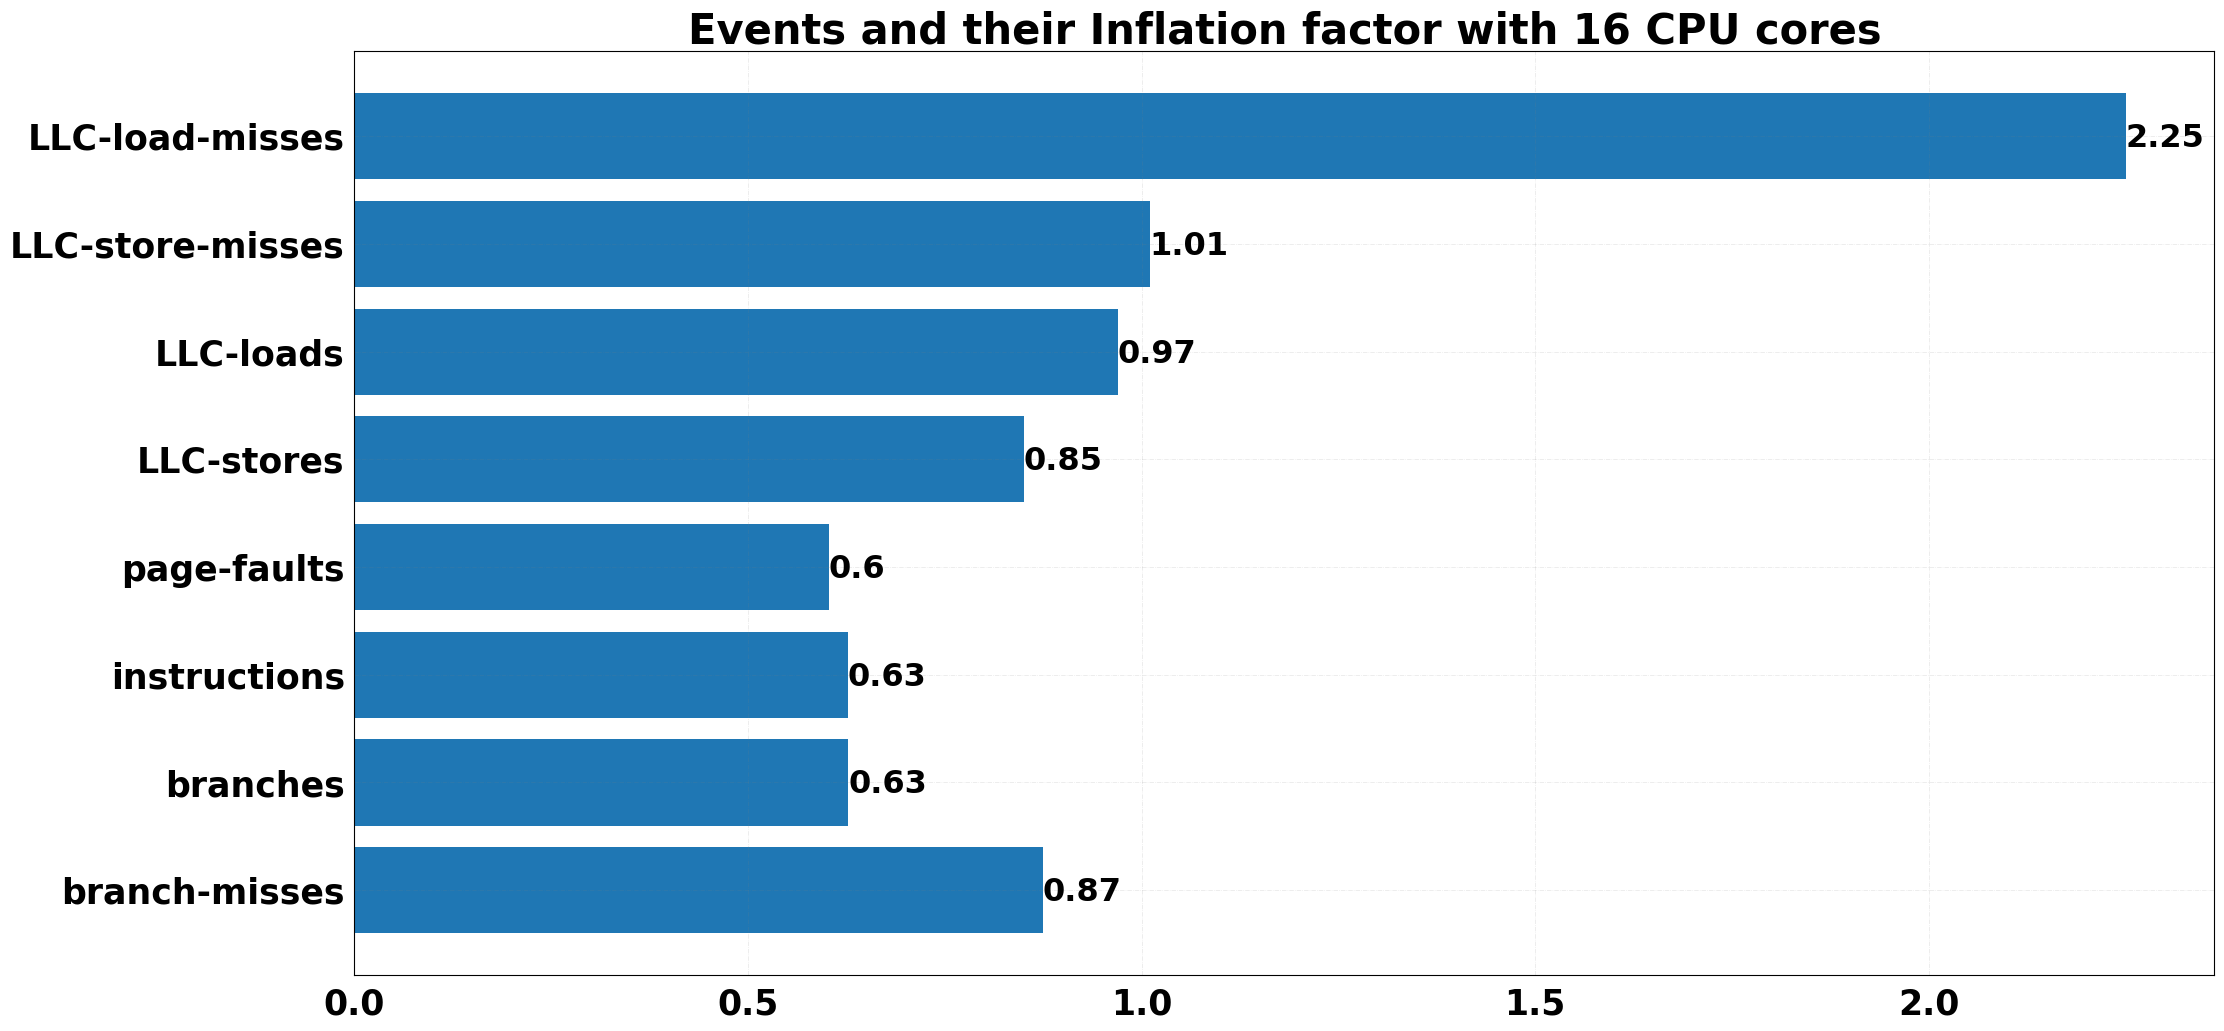
\includegraphics[width=\linewidth]{Images/perf_evalpro_application.png}
  \caption{Inflation factor of Events in Evalpro application by Perf tool}
  \label{perf_results_application}
\end{figure}





The Inflation factor calculated with 16 CPU cores for LLC-load-miss and LLC-store-miss events is compared between  the initial baseline experiments and the final baseline experiments. As shown in the figure \ref{cache_inflation_relation}, when the CPU cache size is increased to more than twice i.e to 49MB from 20MB, the value of $Inflation\_factor(16)$ reduced by more than half for both LLC load and LLC store misses. From these results, it is clear that when the CPU cache size is increased then the Inflation factor reduced proportionally to the CPU cache size

The observed value of the throughput with 16 CPU cores is compared between  the initial baseline experiments and the final baseline experiments shown in sections \ref{baseline_16} and \ref{baseline_64}, respectively. As shown in the figure \ref{throughput_cache_graph}, in our initial baseline experiments  when 16 CPU cores are using 20MB CPU cache, then the observed  throughput, $Throughput_{max}(16)$ was 3.4 requests per second. Using the CPU  and the CPU cache of the same family, in our final  baseline experiments, for 16 CPU cores when the CPU cache size is increased to more than twice i.e, to 49MB from 20MB, then the observed  throughput, $Throughput_{max}(16)$ was 8.75 requests per second i.e throughput increased to more than twice. From these results it is clear that when the CPU cache size is increased then the throughput increased proportionally to the CPU cache size.

\begin{figure}[!htb]
  \centering
  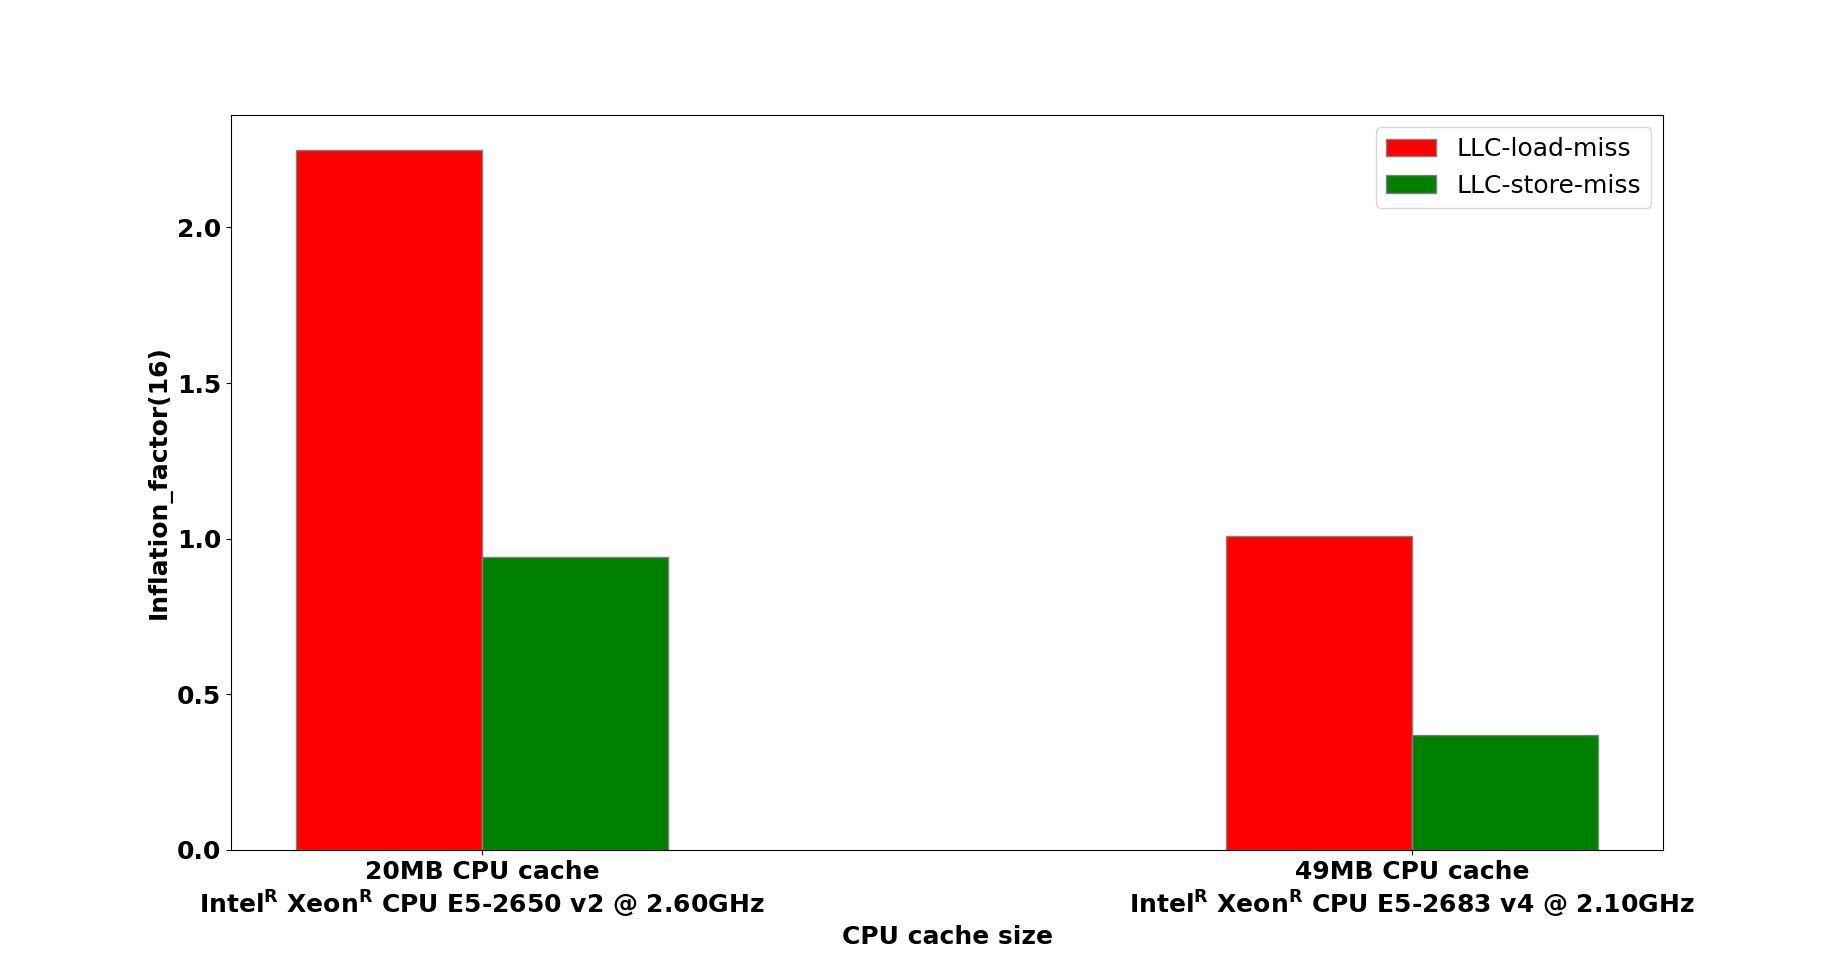
\includegraphics[width=\linewidth]{Images/llc-misses_vs_cache_size.png}
  \caption{Inflation factor of LLC misses vs CPU cache size }
  \label{cache_inflation_relation}
\end{figure}


Using the table \ref{tab:cache_summary_performance}, we have summarized the above results. By which, it is clear that when the CPU cache size increased, the number of L3 load misses and L3 store miss decreased proportionally. As a result, the throughput of the Evalpro application increased proportionally with the CPU cache size. Therefore our hypothesis that the  CPU cache is the bottleneck for the Evalpro application turns out to be true.

For our Evalpro application, linear scaling of throughput can be achieved by increasing the number of CPU cores only up to certain number of CPU cores After that since the L3 CPU cache is shared among the CPU cores,  due to memory intensive nature of the Evalpro application,the cache misses have disproportionately inflated . Due to which the throughput of the Evalpro application didn't scale linearly by increasing the number of CPU cores. Hence to get the linear scaling of the throughput, CPU cache size also should be incremented with the CPU cores. The next chapter recommends the minimum L3 CPU cache size required for a certain number of CPU cores to achieve linear scaling of the throughput for the Evalpro application.

\begin{figure}[!htb]
  \centering
  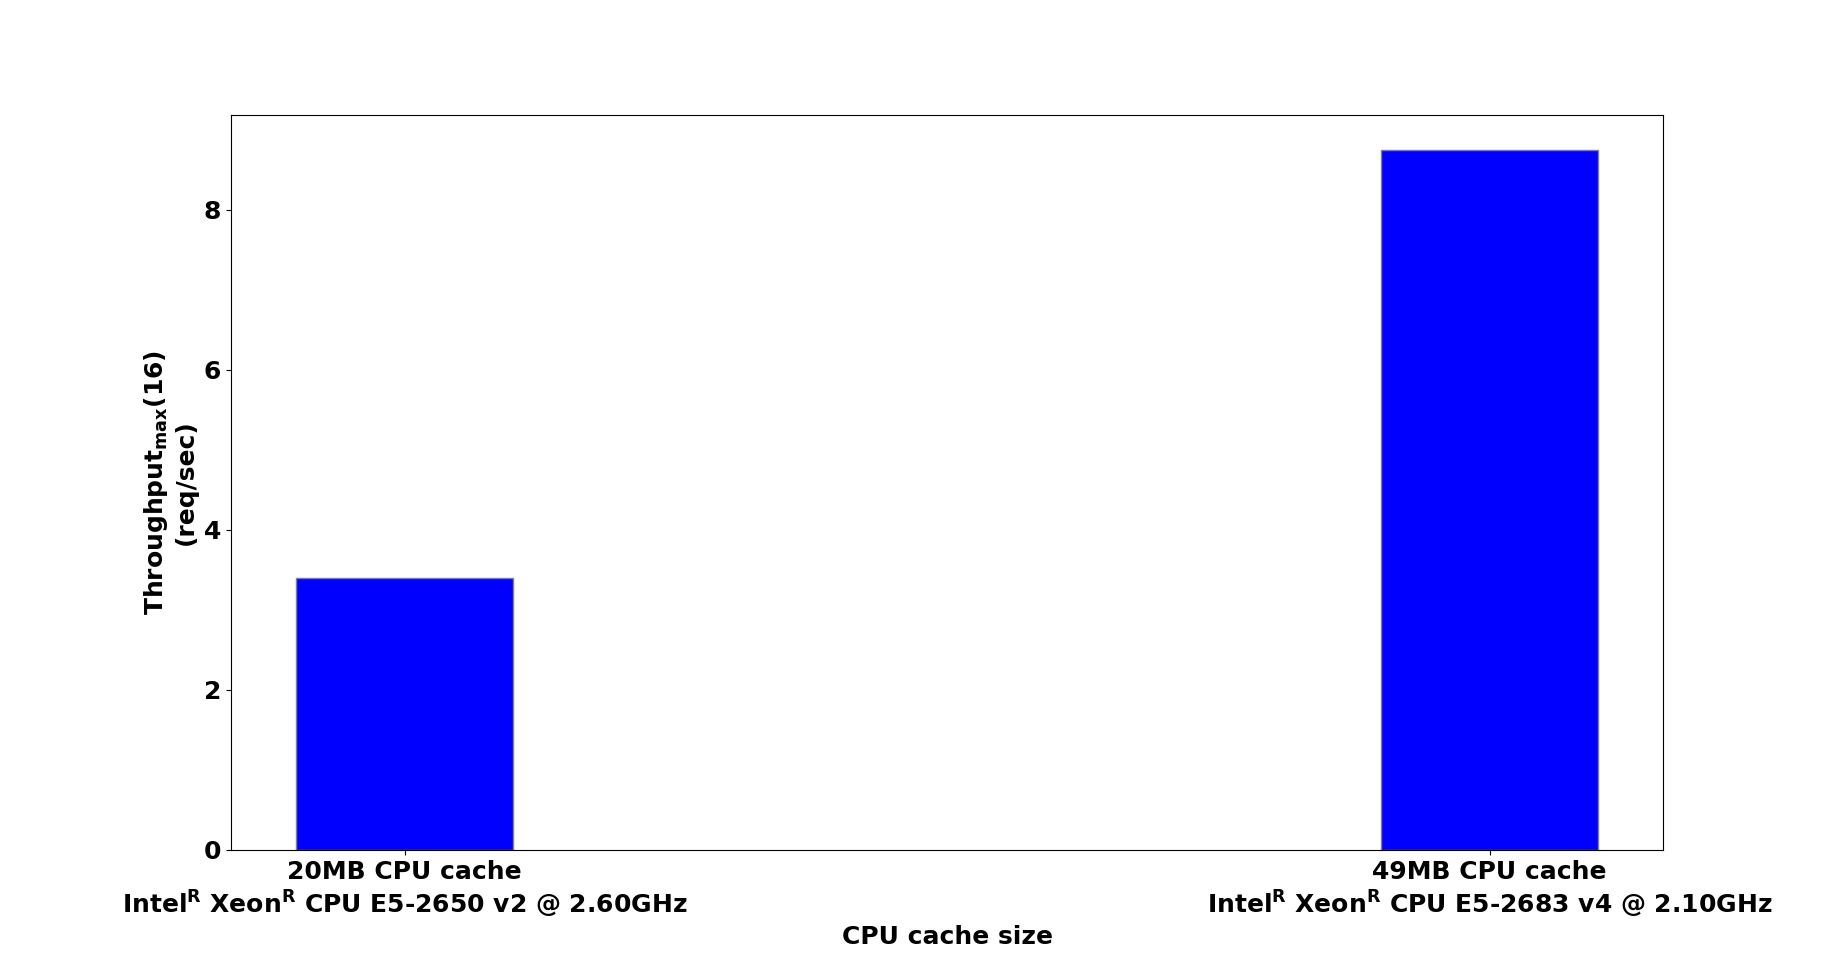
\includegraphics[width=\linewidth]{Images/throughput_vs_cache_size.png}
  \caption{Throughput vs CPU cache size }
  \label{throughput_cache_graph}
\end{figure}




\begin{table}[!htb]
    \centering
     \begin{tblr}{
      colspec={|X[3]|X|X|X|}, row{1} = {c},row{2} = {c}, row{3} = {c}, hlines,
    }
    &\makecell{Baseline - 16}&\makecell{Baseline - 64}& \makecell{\% of \\ increase or \\decrease}\\
    \makecell{CPU cache size for \\ 16 CPU cores} & \makecell{20 MB} & \makecell{49 MB}&\makecell{+ 145}\\
    \makecell{$Inflation_factor_{LLC-load-misses}(16)$} & \makecell{2.25} & \makecell{0.94}&\makecell{- 140}\\
    \centering{\makecell{$Inflation_factor_{LLC-store-misses}(16)$}} & \makecell{1.01} & \makecell{0.37}&\makecell{- 170}\\
    \makecell{$Throughput_{max}(16)$ \\ (req/sec)} & \makecell{3.37} & \makecell{8.75}&\makecell{+ 160}\\
    \end{tblr}
\caption{Summary of the CPU Cache size affect on the performance of the Evalpro application}
  \label{tab:cache_summary_performance}
\end{table}


\chapter{Recommendations for Linearly Scaling Evalpro}\label{evalpro_recommendation}

Using the Baseline-16 and Baseline-64 experiment results described in the sections \ref{baseline_16} and \ref{baseline_64}, respectively,in this chapter, we found  the minimum L3 CPU cache size required for a certain number of CPU cores to achieve linear scaling of the throughput.

\begin{equation}
   Per \; core \; L3 \; cache =\frac{L3  \; CPU  \; cache  \; size}{Number \; of  \; CPU  \; cores}
  \label{eq:3}
\end{equation}


From the Baseline-16 experiments described in the section \ref{baseline_16}, we found that when the number of CPU cores $N>8$, the throughput scaling of the Evalpro application is not linear. Since the L3 CPU cache size for Baseline-16 is 20MB, using equation \ref{eq:3}, we can say that when the number of CPU cores $N>8$, the  Per core L3 cache is less than 2.5. Therefore we can say that  the throughput is not scaling linearly when the Per core L3 cache is less than 2.5.

Similarly, from the Baseline-64 experiments described in the section \ref{baseline_64}, we found that when the number of CPU cores $N>16$, the throughput scaling of the Evalpro application is not linear. Since the L3 CPU cache size for Baseline-64 is 40MB for 32 CPU cores, using equation \ref{eq:3}, we can say that when the number of CPU cores $N>16$, the Per core L3 cache is less than 2.5. Therefore we can say  the throughput is not scaling linearly when the Per core L3 cache is less than 2.5.

\begin{table}[!htb]
    \centering
  \begin{tabularx}{\textwidth}{|X|X|}
    \hline
    \makecell{Number of CPU cores}&\makecell{Minimum L3 cache required \\ for Linear scaling of throughput}\\
    \hline
    \makecell{8} & \makecell{20 MB}\\
    \hline
    \makecell{16} & \makecell{40 MB}\\
    \hline
    \makecell{32} & \makecell{80 MB}\\
    \hline
    \makecell{64} & \makecell{160 MB}\\
  \hline
\end{tabularx}
\caption{Cache size required for Linear scaling of the throughput with CPU cores}
  \label{tab:cpu_cache_cores}
\end{table}

From the above results, we can say that for our Evalpro application to achieve linear scaling of the throughput with the CPU cores, the minimum value of the Per core L3 cache is 2.5. The table \ref{tab:cpu_cache_cores} shows the minimum L3 CPU cache required for a particular number of CPU cores to achieve linear scaling in the throughput with CPU cores. We conclude the thesis in the next chapter




\chapter{Conclusion}\label{conclusion}
To achieve the goal of linear scaling of the throughput with CPU cores for Evalpro application, we have started with the baseline experiments and found that our Evalpro application's throughput scaling is not proportional to the increase in the CPU cores. Therefore we tried to find the bottlenecks limiting the scalability in the baseline setup and found no application bottlenecks. After that, we tried horizontal scaling for better isolation, in which we tried Container-based virtualization using docker swarm, Hardware-assisted virtualization using KVM-QEMU and used MongoDB in place of the disk to store the files but got no improvement in the scalability. 

We developed two micro benchmarks, i.e., CPU micro benchmark and Evalpro micro benchmark, to find the best scalability that can be achieved for a raw CPU workload and the Evalpro like workload, respectively. We found that the throughput scalability of the Evalpro micro benchmark and the Evalpro application is almost the same. Hence  we performed low level bottleneck analysis on the Evalpro micro benchmark to  reason for its scalability limitation. We used the PERF tool and found that when the number of CPU cores is high, due to g++ compilation, L3 CPU cache misses have been disproportionately inflated. Hence, we hypothesised that the CPU cache size could be the bottleneck for the Evalpro application. 

To validate the above hypothesis, we used the PERF tool on the Evalpro application. We found that for the Evalpro application, L3 load misses are inflated when the number of CPU cores is high. We also found that by increasing  CPU cache size, the number of L3 CPU cache load and store misses have reduced proportionally. As a result of the reduction in the L3 CPU cache misses, the throughput of the Evalpro application increased proportionally with the CPU cache size, which validates our hypothesis that the CPU cache is the bottleneck for the Evalpro application. Therefore we conclude that linear scaling of throughput can be achieved by increasing the number of CPU cores only up to a certain number. After that, to get the linear scaling of the throughput, cache size also should be incremented with the CPU cores.


\begin{figure}[!htb]
  \centering
  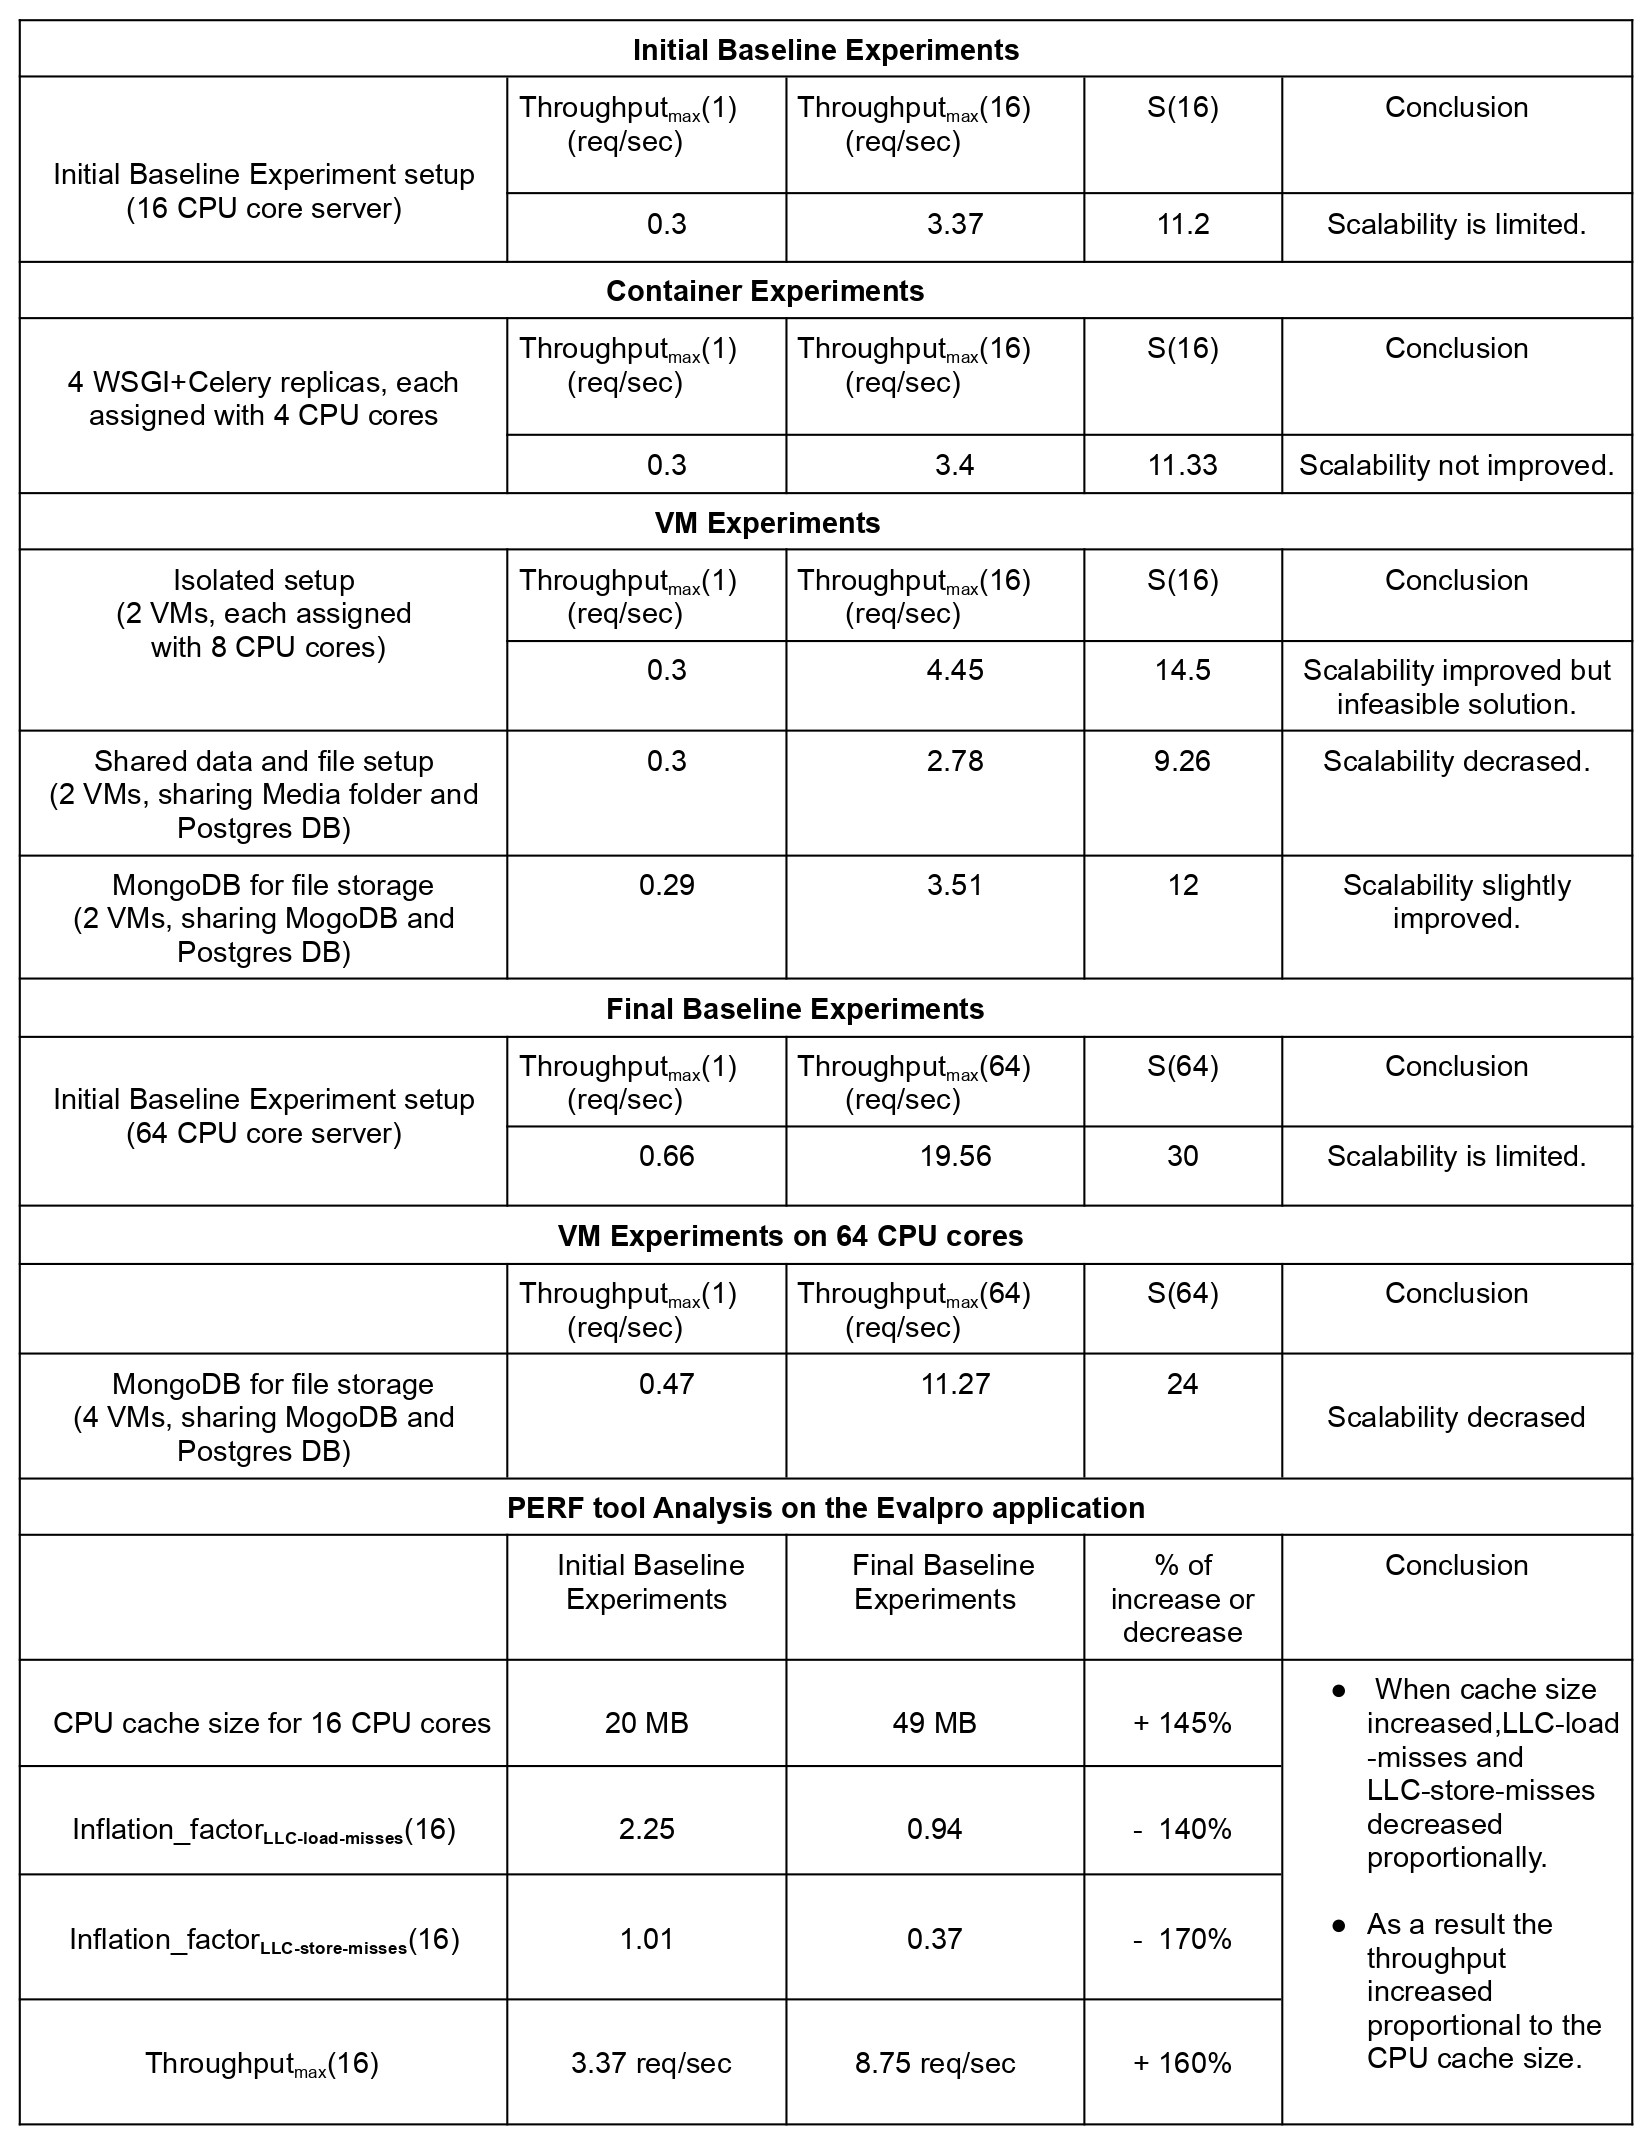
\includegraphics[width=\linewidth]{Images/experiment_summary.jpg}
  \caption{Experiment results Summary }
  \label{paper_summary}
\end{figure}

The table \ref{paper_summary}, shows the results summary of various experiments described.



%****************************************************************
%                         Appendices                           
%****************************************************************
%% Additional, supporting material, such as codes, derivations, etc., can be placed in the appendix

\appendix
\chapter{Load generation and Performance measurement scripts }
In this chapter we discuss about the following  scripts used in the Load generation and Performance measurement infrastructure.

\begin{enumerate}
    \item 
    load\_test.sh
    \item
    scripts.sh
    \item
    post\_processing.sh
\end{enumerate}

\section{load\_test.sh}

The code for load\_test.sh is shown in listing \ref{lst:load_test_sh}, which runs on the client machine, triggers request load to the server using JMeter, and collects all the performance metrics after the load test is completed. Line \ref{line:linux_utilities_start} triggers the execution of scripts.sh in the server machine, which runs Linux utilities in the background and collects snapshots of the load test periodically. We will discuss about scripts.sh in the next section. Line \ref{line:jmeter_use} runs the JMeter script which starts the request load on the Evalpro instance running in the server. After the load generation by the JMeter is completed, line \ref{line:linux_utilities_stop} stops the execution of scripts.sh. Line \ref{line:post_processing_start}, starts the post\_processing.sh script in the server, which uses the snapshots collected by scripts.sh and summarizes the performance metrics by using arithmetic calculations. We will discuss about post\_processing.sh in the next section. Line \ref{line:files_transfer_server1} and the line \ref{line:files_transfer_server2} transfers all the files from the server which contains the summary of the performance metrics. At the end, in the line \ref{line:graph_generator}, using all the files collected, the graphs will be generated which represent the correlation between  different performance metrics.



\lstset{language=bash}
\lstset{frame=lines}
\lstset{breaklines=true}
\lstset{caption={load\_test.sh script}}
\lstset{label={lst:load_test_sh}}
\lstset{basicstyle=\ttfamily,
  showstringspaces=false,
  commentstyle=\color{red},
  keywordstyle=\color{blue}
}
\lstset{numbers=left,
    stepnumber=1}
    


\begin{lstlisting}[escapechar=|]
#!/bin/bash
declare -a timestamp_arr
TIMESTAMP1=`date +%d%m%Y_%H%M%S`
server_metrics_path="server_metrics/${TIMESTAMP1}"
perf_analysis_path="perf_analysis/${TIMESTAMP1}"
if [ ! -d $server_metrics_path ]
then
		mkdir $server_metrics_path
fi
if [ ! -d $perf_analysis_path ]
then
                mkdir $perf_analysis_path
fi
user_vals=( 180,220 )
for i in "${user_vals[@]}"
do
	TIMESTAMP=`date +%d%m%Y_%H%M%S`
	timestamp_arr[$i]=${TIMESTAMP}
	echo "run started"
	sshpass -p "panda123" ssh panda@10.129.131.6 "cd LoadTest;./scripts.sh $i ${timestamp_arr[i]} &" &  |\label{line:linux_utilities_start}|
	echo "Number of users : ${i}"
	sed -i -E "s/\"ThreadGroup.num_threads\">([0-9]+)/\"ThreadGroup.num_threads\">${i}/g" evalpro_load_test.jmx
	path="test_results/users_${i}_${TIMESTAMP}"
	if [ ! -d $path ]
	then
		mkdir $path
	fi
	/home/panda/LoadTest/ClientFolder/rnd_load_test/apache-jmeter-5.3/bin/jmeter -n -t evalpro_load_test.jmx -l $path/results.csv -e -o $path/output |\label{line:jmeter_use}|

	sshpass -p "panda123" ssh panda@10.129.131.6 "ps -ef | grep -v grep | grep scripts.sh | awk '{print \$2}' | xargs kill" |\label{line:linux_utilities_stop}|
    echo "experiment done"
	sleep 60
	if [ -f jmeter.log ]
	then
		mv jmeter.log $path/
	fi
done
echo "post processing started"
n_server_cores=`sshpass -p "panda123" ssh panda@10.129.131.6 "nproc"`
for i in "${user_vals[@]}"
do
	sshpass -p "panda123" ssh panda@10.129.131.6 "cd LoadTest; ./post_processing.sh $i ${timestamp_arr[i]}" |\label{line:post_processing_start}|
	sshpass -p "panda123" scp -r panda@10.129.131.6:/home/panda/LoadTest/metrics/*$i_${timestamp_arr[i]}* /home/panda/LoadTest/ClientFolder/rnd_load_test/${server_metrics_path}/ |\label{line:files_transfer_server1}|
	sshpass -p "panda123" scp -r panda@10.129.131.6:/home/panda/LoadTest/timeseries_metrics/*$i_${timestamp_arr[i]}*/* /home/panda/LoadTest/ClientFolder/rnd_load_test/${perf_analysis_path}/ |\label{line:files_transfer_server2}|
	cp test_results/users_${i}_${timestamp_arr[i]}/output/statistics.json /home/panda/LoadTest/ClientFolder/rnd_load_test/${server_metrics_path}/client_side_values_${i}.json
	python3 server_metrics_extract.py /home/panda/LoadTest/ClientFolder/rnd_load_test/${server_metrics_path} ${n_server_cores} |\label{line:graph_generator}|
done 
echo "post processing completed"
\end{lstlisting}



\section{scripts.sh}
The code for scripts.sh is shown in listing \ref{lst:scripts_sh}, which executes on the server machine, and runs the Linux utilities in background. It periodically collects the snapshots of the server during the load test. It gets triggered for execution before the load test is started by the load\_test.sh, described in the previous section. As shown in  listing \ref{lst:scripts_sh}, during the load test, the snapshots of Linux utilities, i.e , ps, iostat, netstat, mpstat, vmstat and iotop are collected in the background. At the end, in the line \ref{line:wait_linux_utilities}, the  scripts.sh waits until all the Linux utilities have completed the collection of snapshots.


\lstset{language=bash}
\lstset{frame=lines}
\lstset{breaklines=true}
\lstset{caption={scripts.sh script}}
\lstset{label={lst:scripts_sh}}
\lstset{basicstyle=\ttfamily,
  showstringspaces=false,
  commentstyle=\color{red},
  keywordstyle=\color{blue}
}
\lstset{numbers=left,
    stepnumber=1}
    
\lstset{ escapeinside={(*@}{@*)}},

\begin{lstlisting}[escapechar=|]
#!/bin/bash

cleanup()
{
	kill $p1 $p2 $p3
	exit
}
trap cleanup SIGINT
trap cleanup SIGKILL
trap cleanup SIGTERM

users=$1
TIMESTAMP=$2
snapshot_path="snapshots/users_${users}_${TIMESTAMP}"
mkdir $snapshot_path
ps_scripts/ps.sh > ${snapshot_path}/ps_output_${users}.json &
p1=$!
iostat_scripts/iostat.sh > ${snapshot_path}/iostat_output_${users}.json &
p2=$!
netstat_scripts/net_stat.sh > ${snapshot_path}/netstat_output_${users}.json &
p3=$!
mpstat_scripts/mpstat.sh > ${snapshot_path}/mpstat_output_${users}.json &
p4=$!
vmstat_scripts/vmstat.sh > ${snapshot_path}/vmstat_output_${users}.json &
p5=$!
sudo -u root iotop_scripts/iotop.sh > ${snapshot_path}/iotop_output_${users}.json &
p6=$!

wait $p1 $p2 $p3 $p4 $p5 $p6 |\label{line:wait_linux_utilities}|
\end{lstlisting}


\section{post\_processing.sh}

The code for post\_processing.sh is shown in listing \ref{lst:post_processing_sh}, which executes on the server machine, and runs the scripts which use the snapshots collected by scripts.sh, described in the previous section. Using the snapshots, it summarizes the performance metrics of the server by performing different arithmetic operations i.e average, minimum, and maximum. It gets triggered for execution after the load test is completed by the load\_test.sh, described in the previous section. At the end, in  the line \ref{line:wait_linux_utilities1}, the  post\_processing.sh waits until all the scripts have summarized the performance metrics of the server using the collected snapshots.


\lstset{language=bash}
\lstset{frame=lines}
\lstset{breaklines=true}
\lstset{caption={post\_processing.sh script}}
\lstset{label={lst:post_processing_sh}}
\lstset{basicstyle=\ttfamily,
  showstringspaces=false,
  commentstyle=\color{red},
  keywordstyle=\color{blue}
}
\lstset{numbers=left,
    stepnumber=1}
    
\lstset{ escapeinside={(*@}{@*)}},

\begin{lstlisting}[escapechar=|]
#!/bin/bash
users=$1
TIMESTAMP=$2
path="metrics/users_${users}_${TIMESTAMP}"
mkdir $path
snapshot_path="snapshots/users_${users}_${TIMESTAMP}"
timeseries_metrics_path="timeseries_metrics/users_${users}_${TIMESTAMP}"
mkdir $timeseries_metrics_path
python3 ps_scripts/ps.py  ${snapshot_path}/ps_output_${users}.json $path &
p1=$!
python3 iostat_scripts/iostat.py ${snapshot_path}/iostat_output_${users}.json $path &
p2=$!
python3 netstat_scripts/summary.py ${snapshot_path}/netstat_output_${users}.json $path &
p3=$!
python3 mpstat_scripts/mpstat_metrics_avg.py ${snapshot_path}/mpstat_output_${users}.json $path &
p4=$!
python3 vmstat_scripts/vmstat_avg_metrics.py ${snapshot_path}/vmstat_output_${users}.json $path &
p5=$!
python3 iotop_scripts/iotop.py ${snapshot_path}/iotop_output_${users}.json $path &
p6=$!
python3 iotop_scripts/iotop_avg_metrics.py ${snapshot_path}/iotop_output_${users}.json $path &
p7=$!
python3 vmstat_scripts/vmstat_time_series.py ${snapshot_path}/vmstat_output_${users}.json  $timeseries_metrics_path &
p8=$!
python3 mpstat_scripts/mpstat_time_series.py ${snapshot_path}/mpstat_output_${users}.json  $timeseries_metrics_path &
p9=$!
python3 iotop_scripts/iotop_time_series.py ${snapshot_path}/iotop_output_${users}.json $timeseries_metrics_path &
p10=$!

wait $p1 $p2 $p3 $p4 $p5 $p6 $p7 $p8 $p9 $p10 |\label{line:wait_linux_utilities1}|
\end{lstlisting}


\printbibliography
\addcontentsline{toc}{chapter}{Bibliography}



\end{document}

%%% Local Variables: 
%%% mode: latex
%%% TeX-master: t
%%% End: 
